\chapter{R and RStudio installation}
\label{cha:r-installation}

To install RStudio development environment \cite{rstudio}, first we need to install R from the \acrfull{cran} R project \cite{r-project}.

\section{R installation}

To install R follow the next steps:

\begin{enumerate}
    \item Go to \acrshort{cran} R project website (\url{https://cran.r-project.org/}).
        \begin{figure}[H]
            \centering
            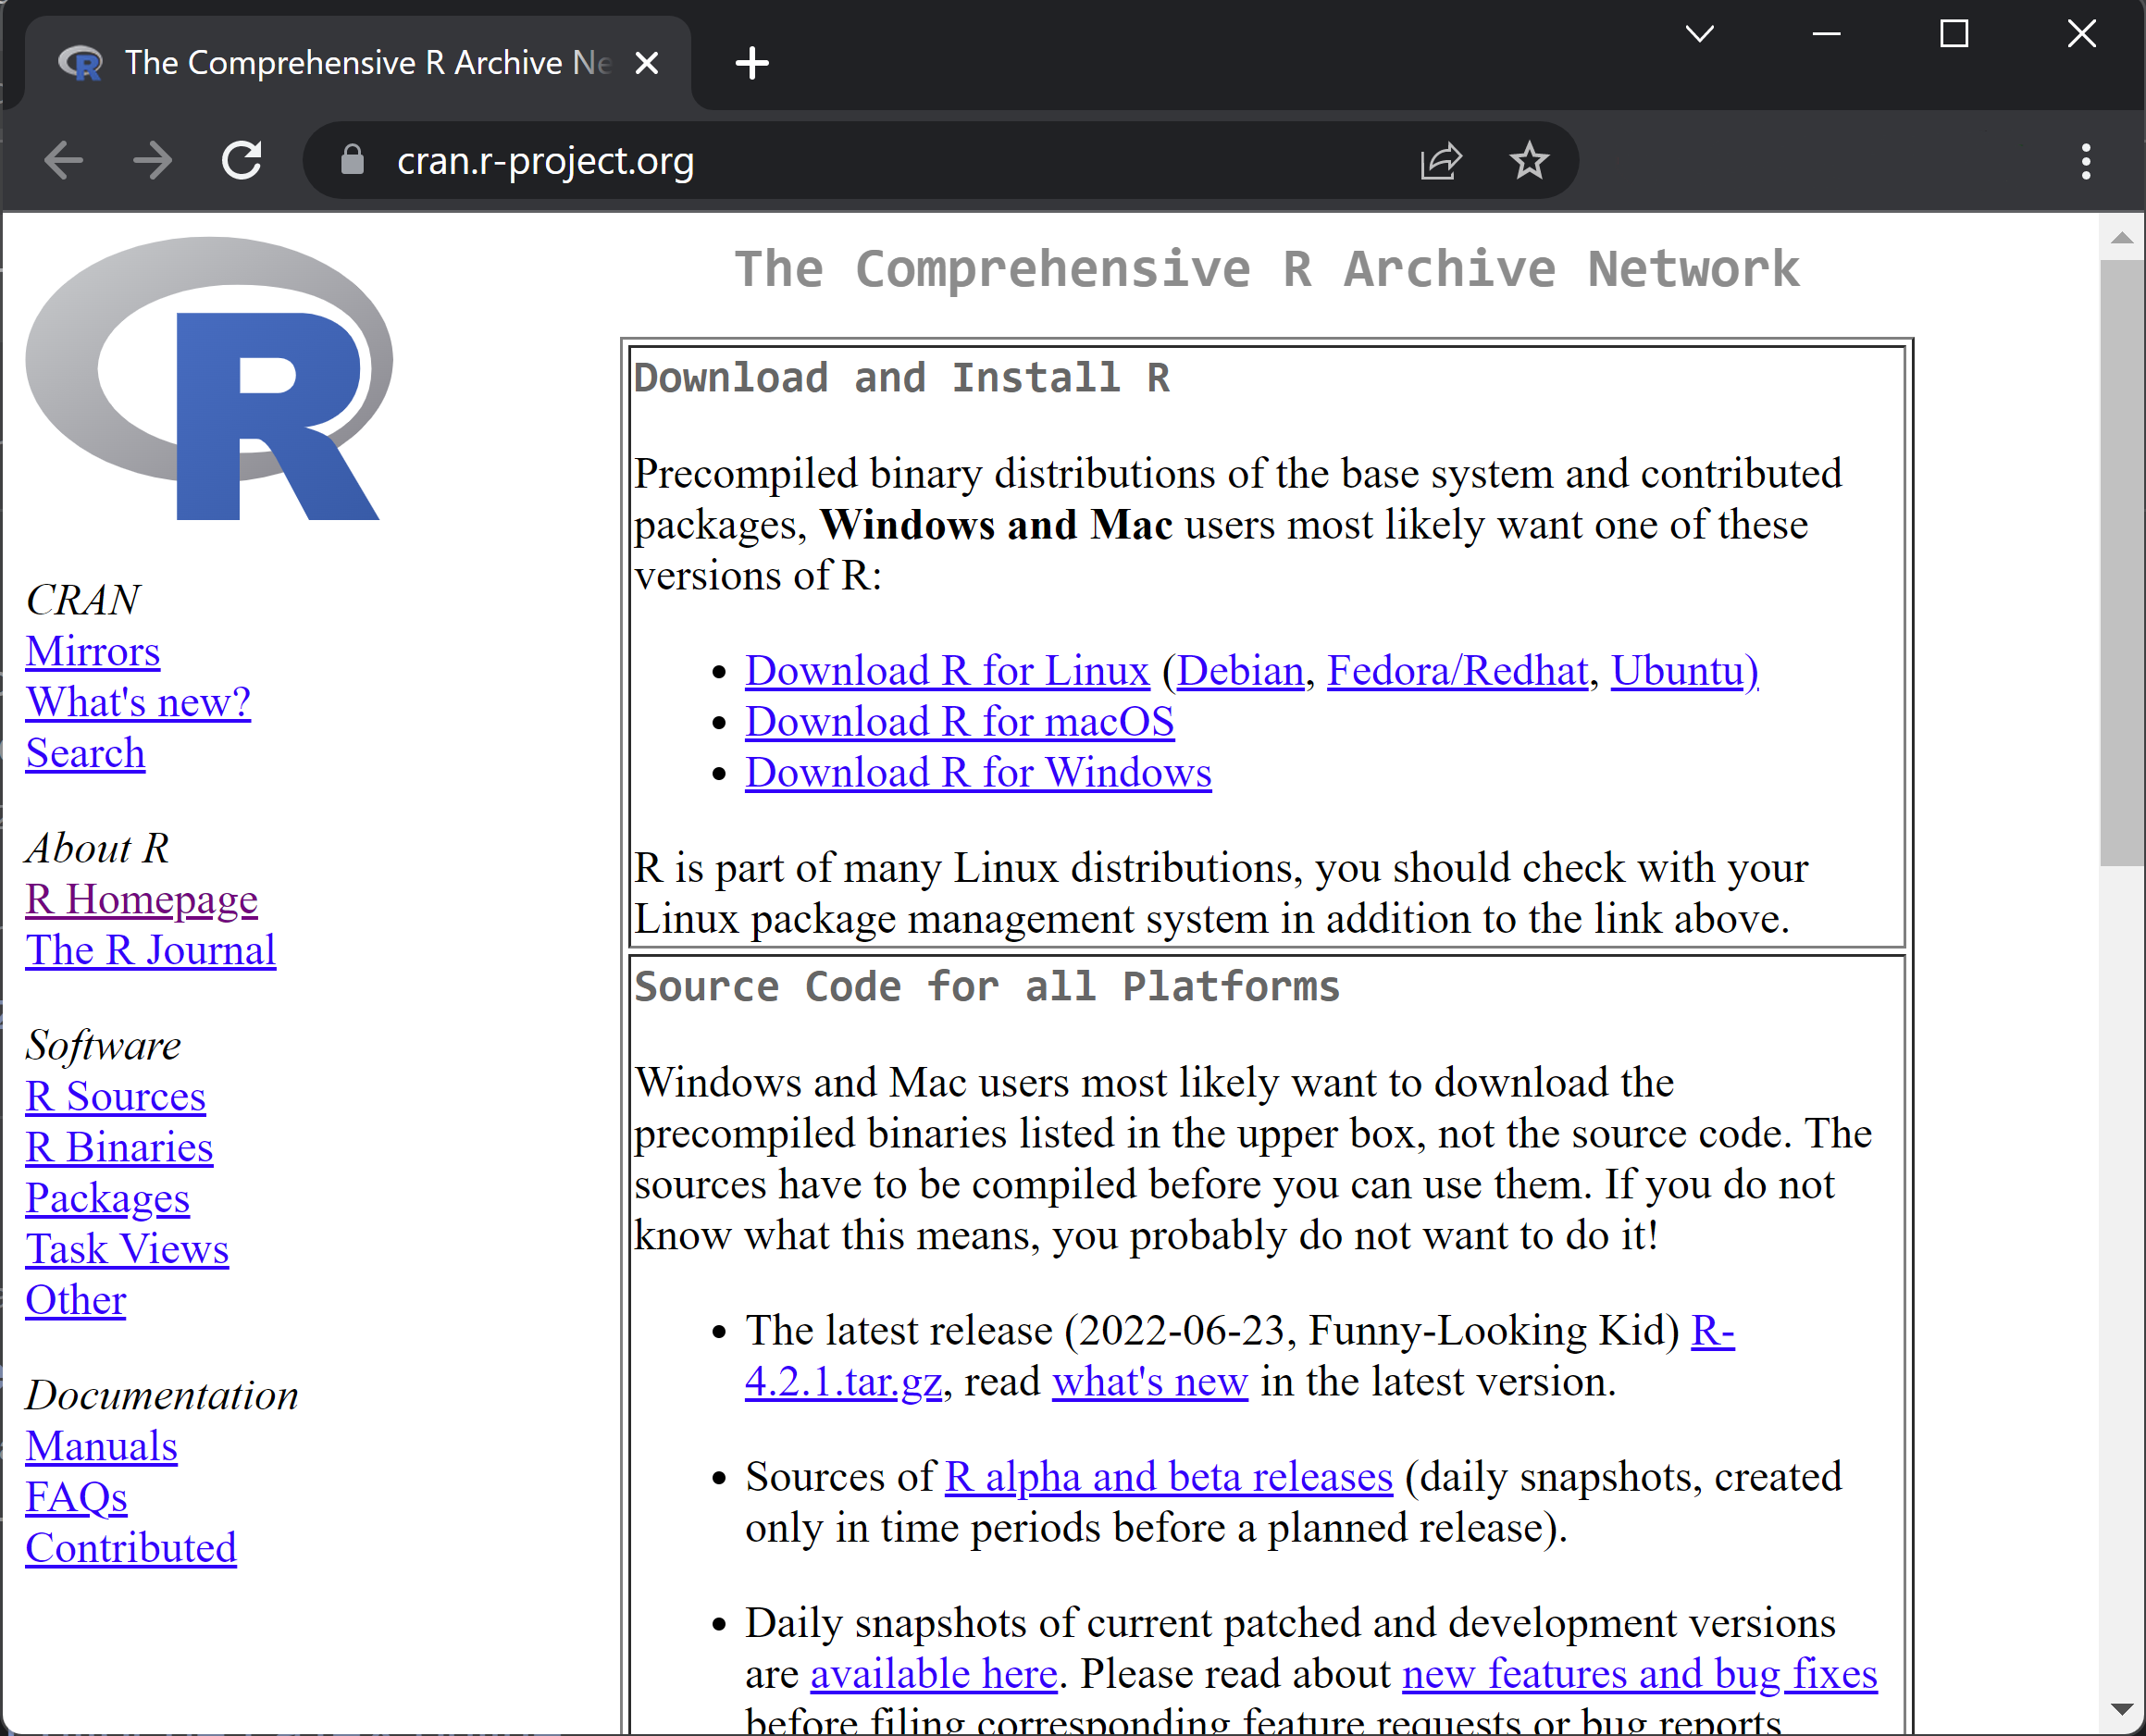
\includegraphics[scale=0.5]{r-installation/cran.png}
            \caption{\acrshort{cran} R project website.}
            \label{fig:cran}
        \end{figure}
    
    \item Click on the \textbf{Download R for Windows} link.
    
    \item Click on the \textbf{install R for the first time} link.
        \begin{figure}[H]
            \centering
            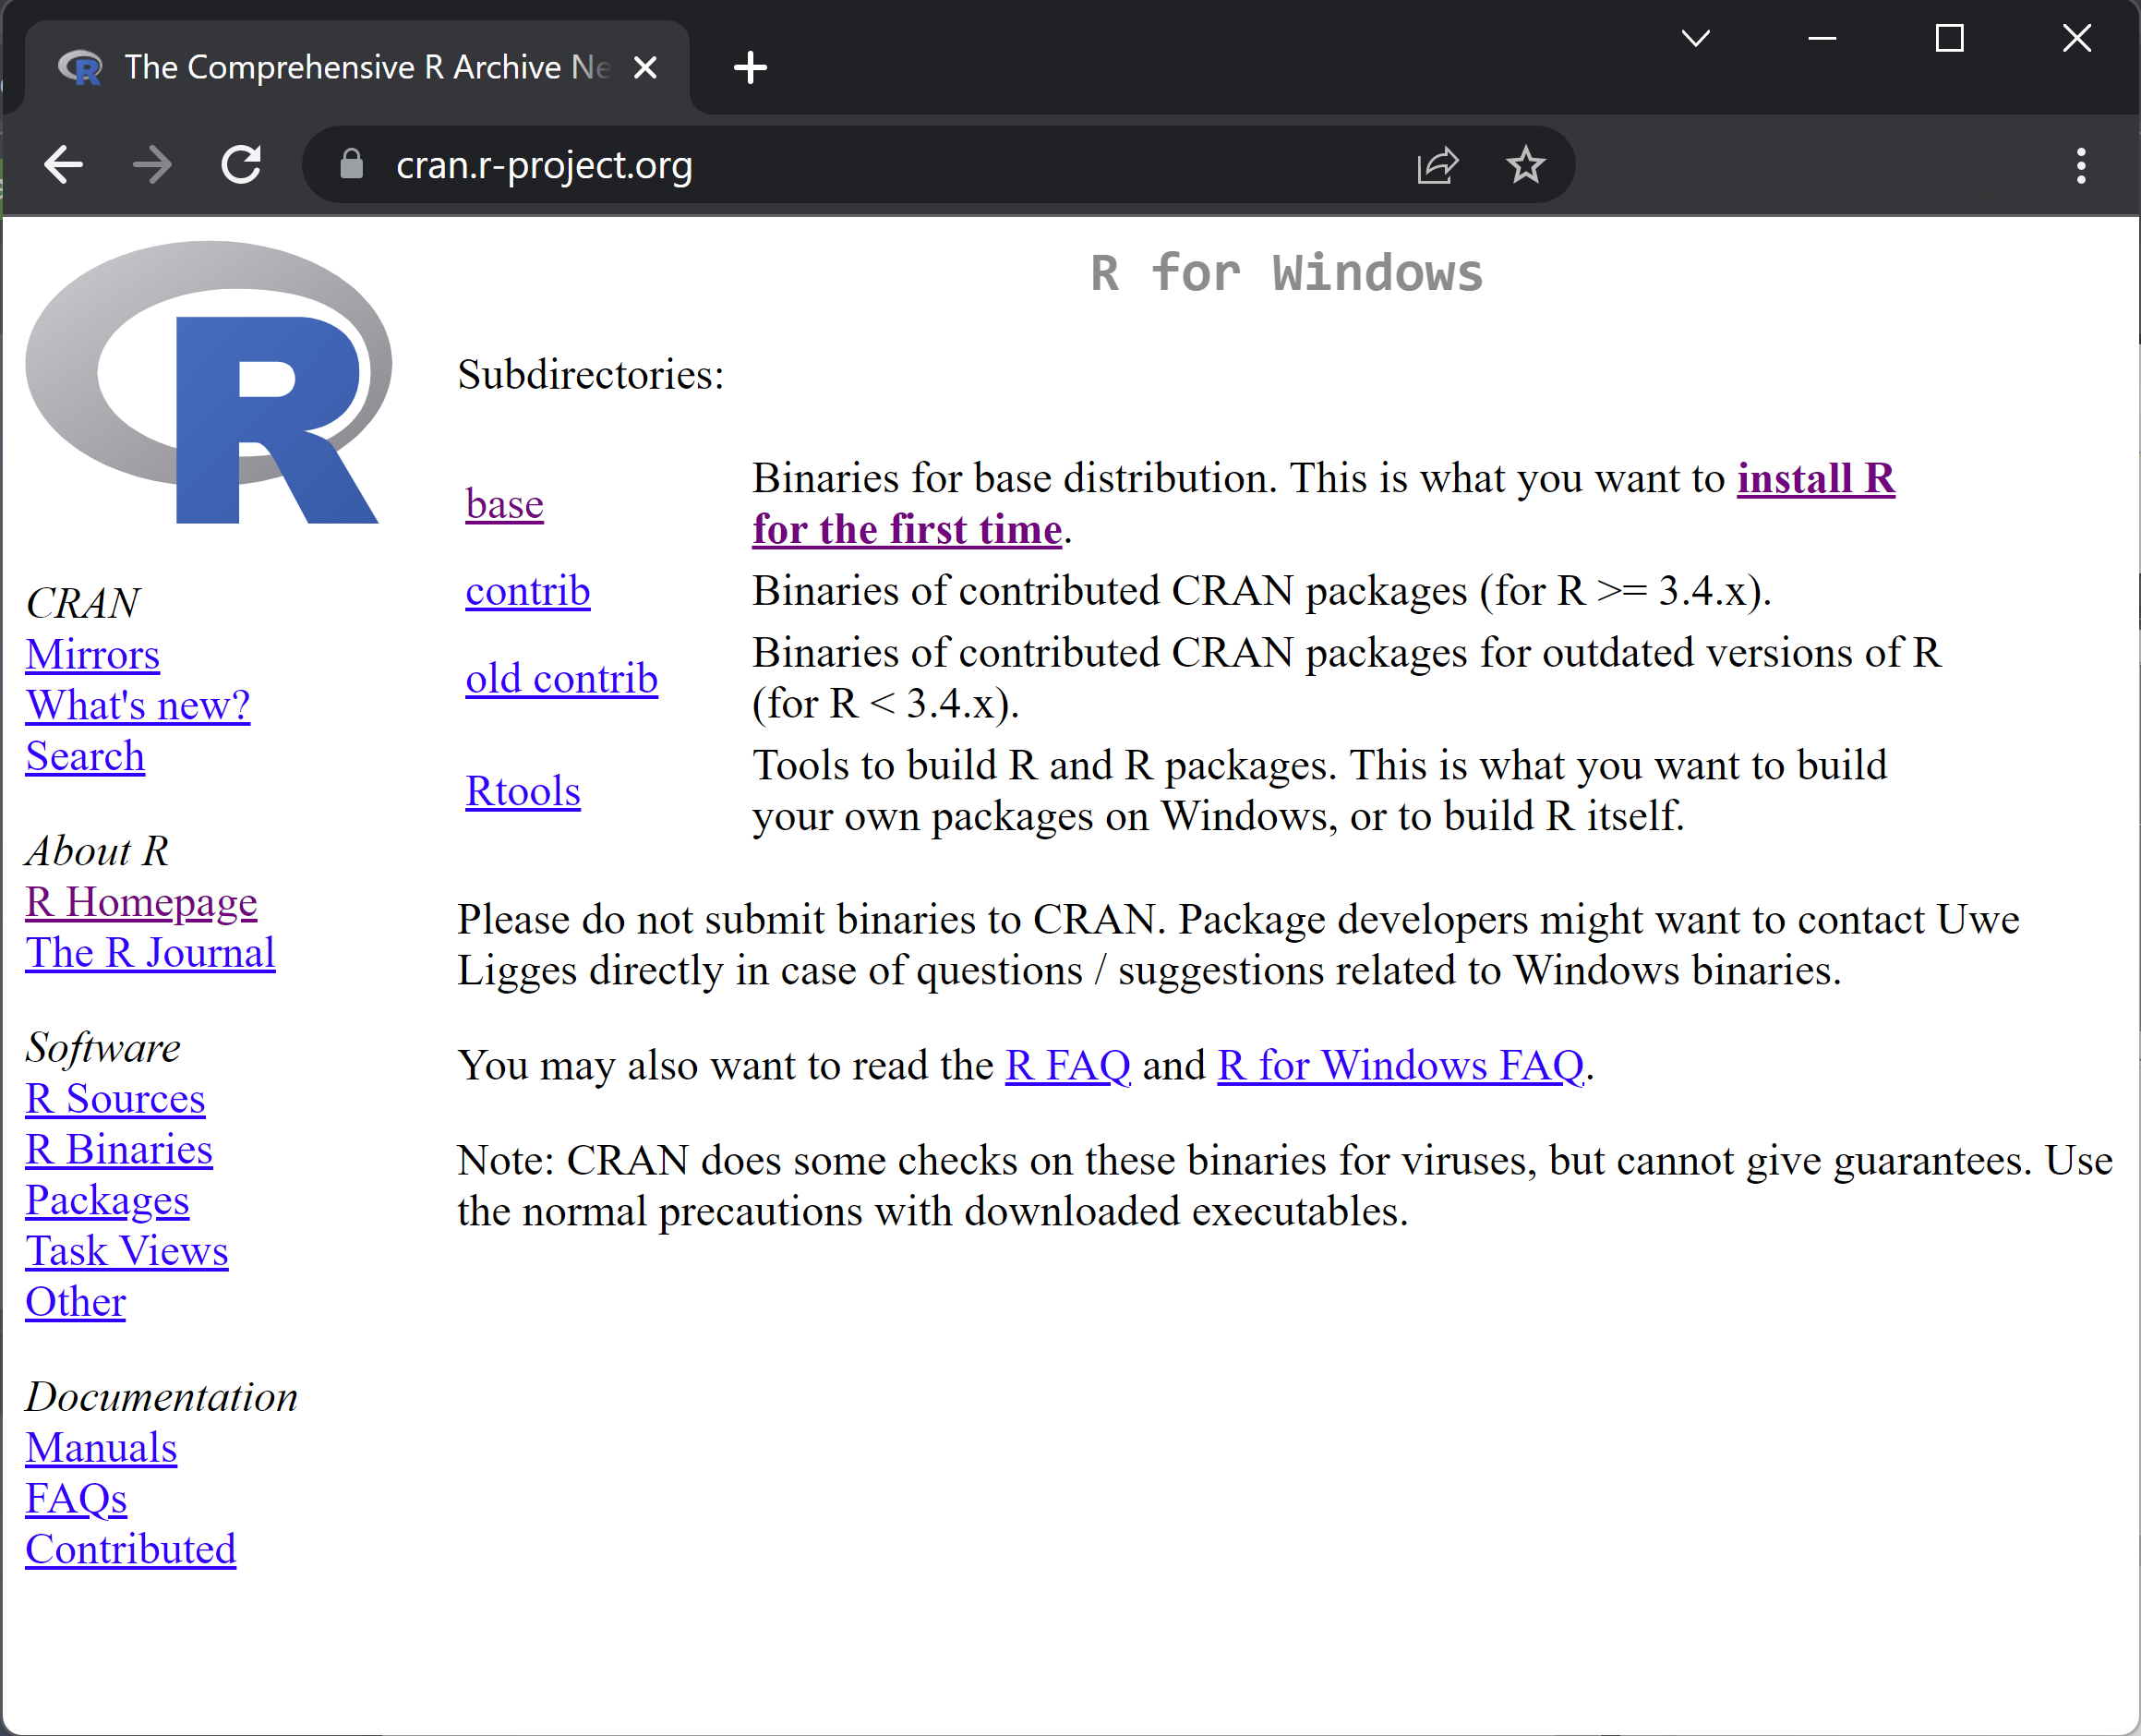
\includegraphics[scale=0.5]{r-installation/r-windows.png}
            \caption{Download R for Windows.}
            \label{fig:r-windows}
        \end{figure}
    
    \item Click \textbf{Download R-4.2.1 for Windows} and save the executable .exe file.
        \begin{figure}[H]
            \centering
            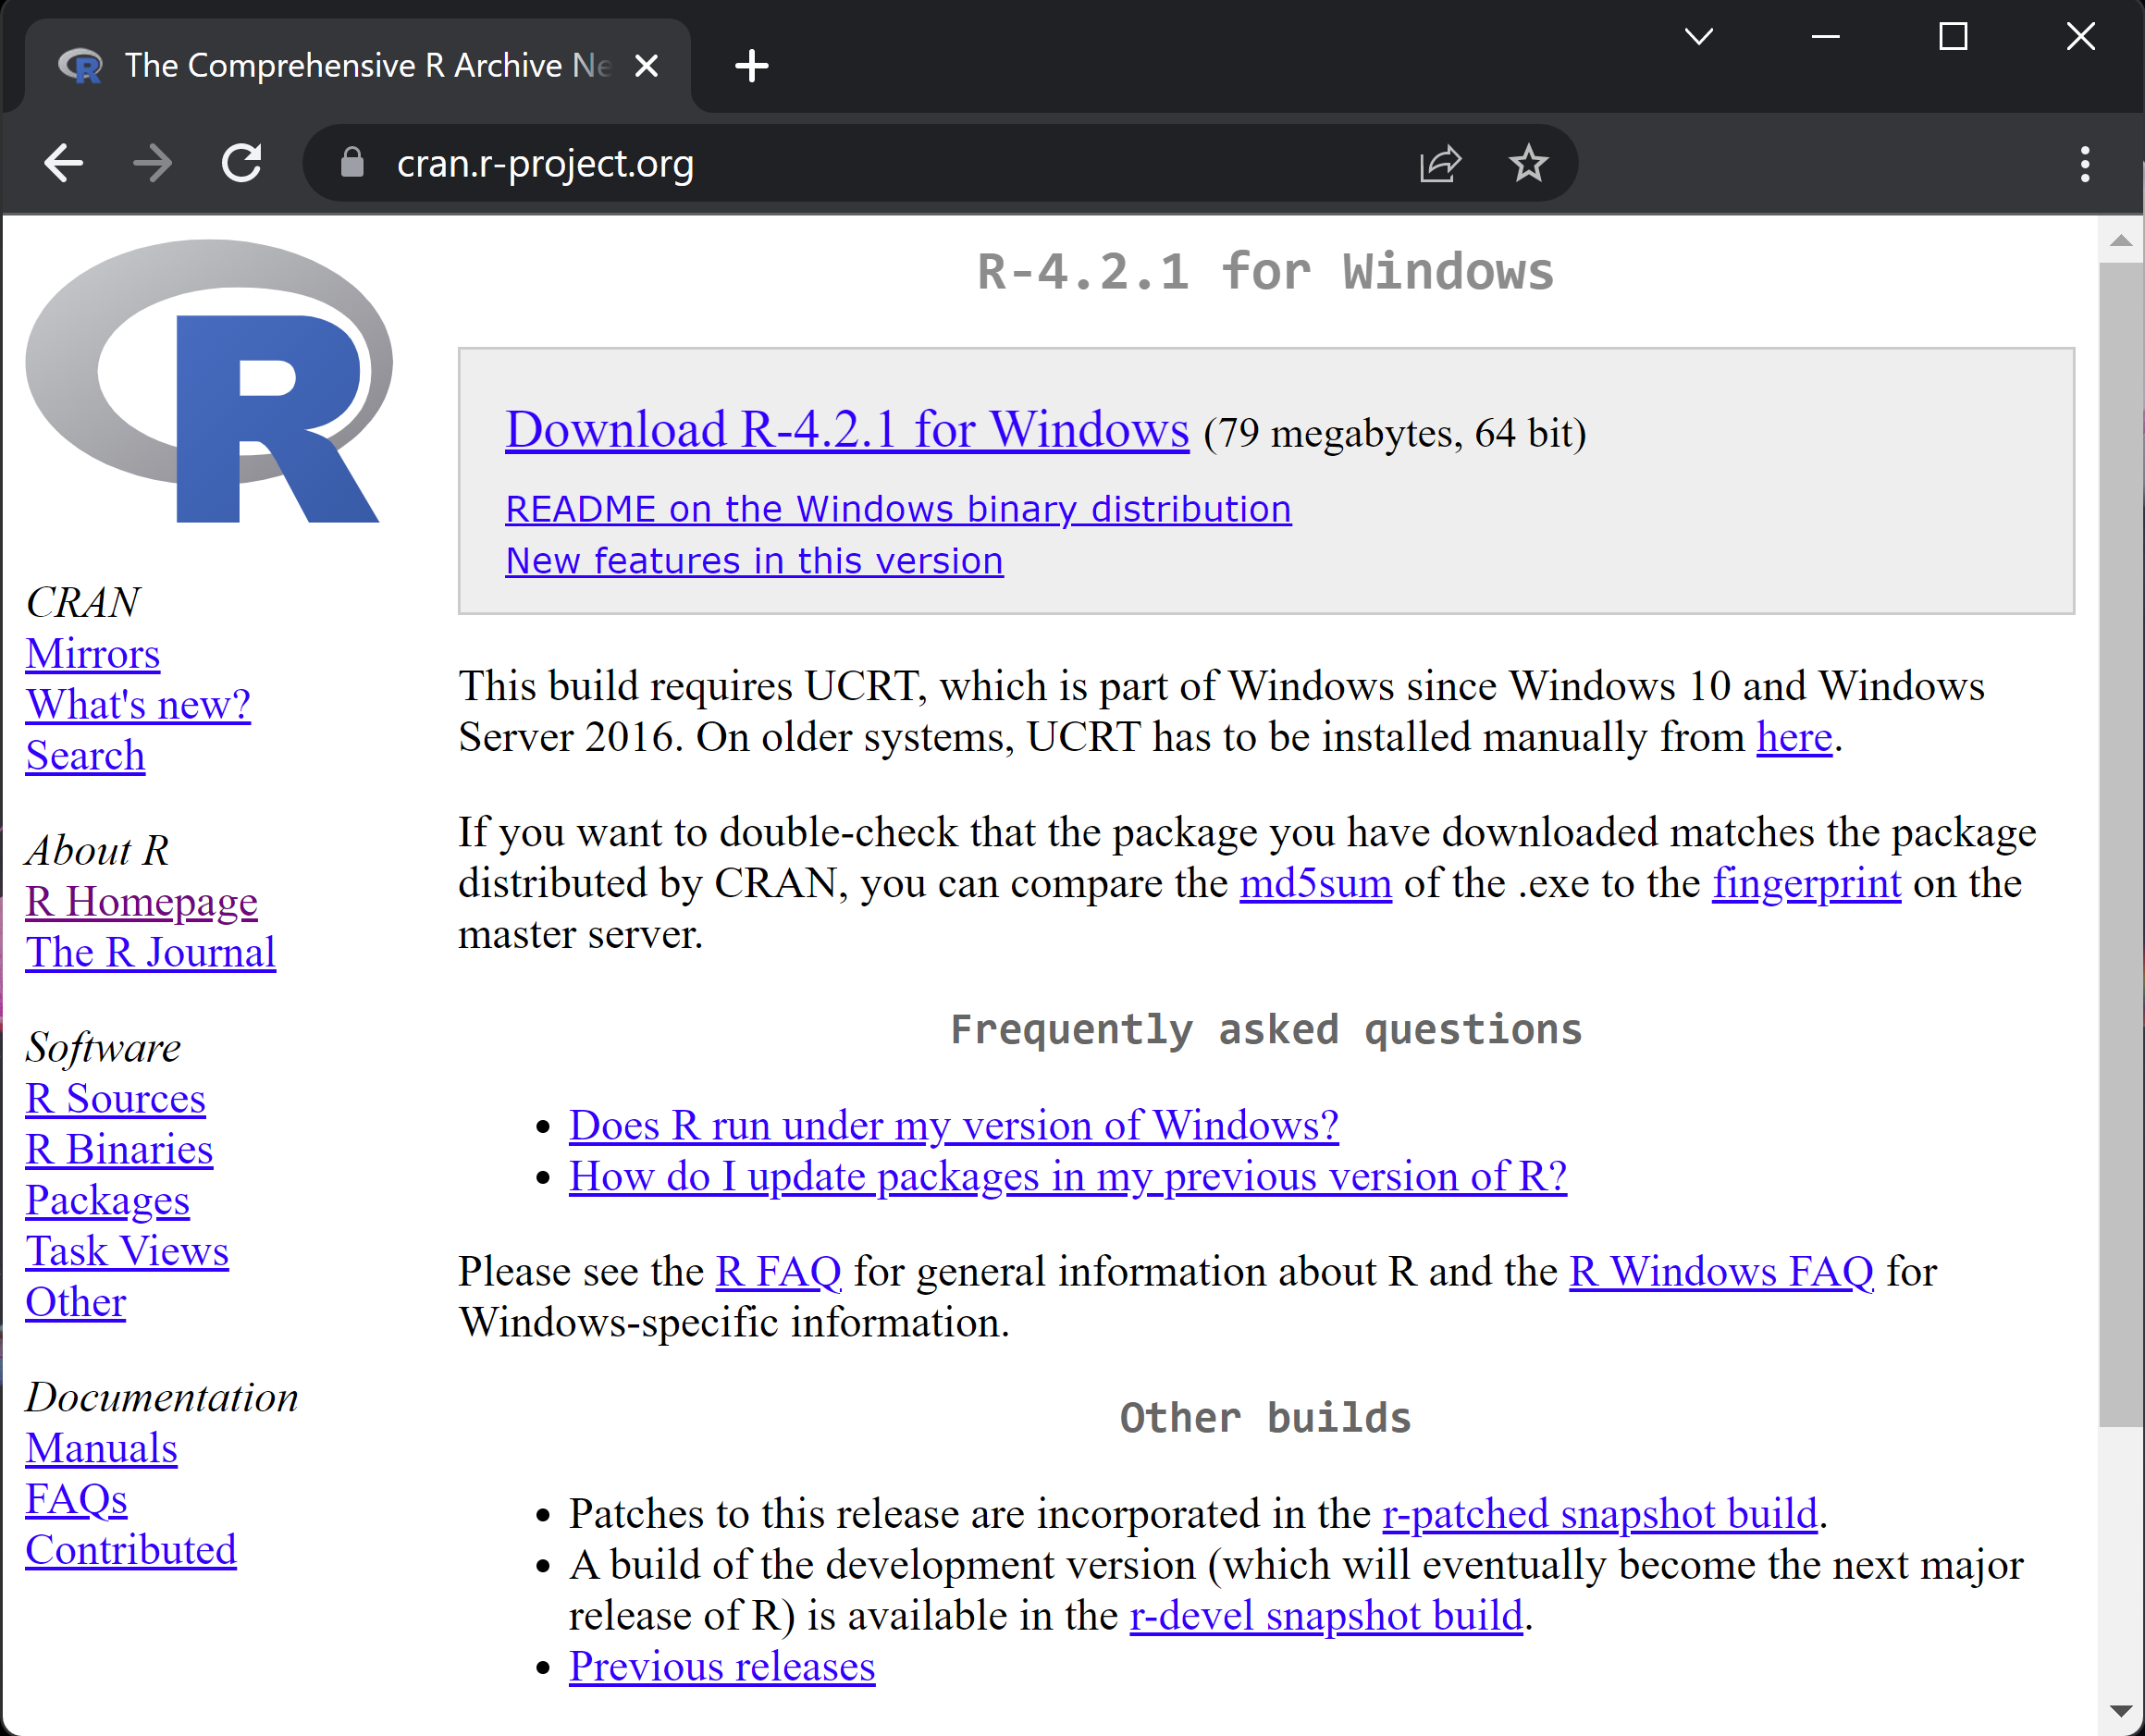
\includegraphics[scale=0.5]{r-installation/download-r.png}
            \caption{Download R latest version.}
            \label{fig:download-r}
        \end{figure}
    
    \item Then, run the .exe file.
    
    \item Choose the language. Click \textbf{Aceptar}.
        \begin{figure}[H]
            \centering
            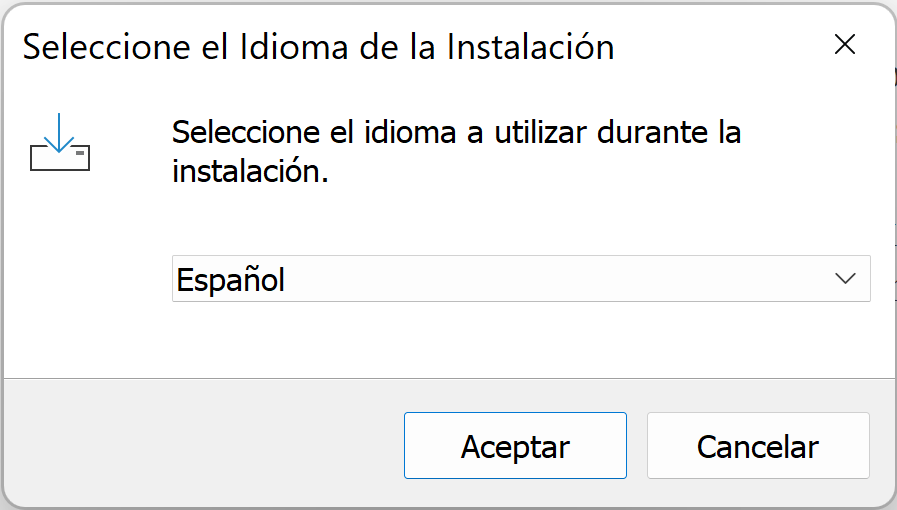
\includegraphics{r-installation/language.png}
            \caption{Choose the language.}
            \label{fig:language}
        \end{figure}
        
    \item Read GNU GENERAL PUBLIC LICENSE and click \textbf{Siguiente}.
        \begin{figure}[H]
            \centering
            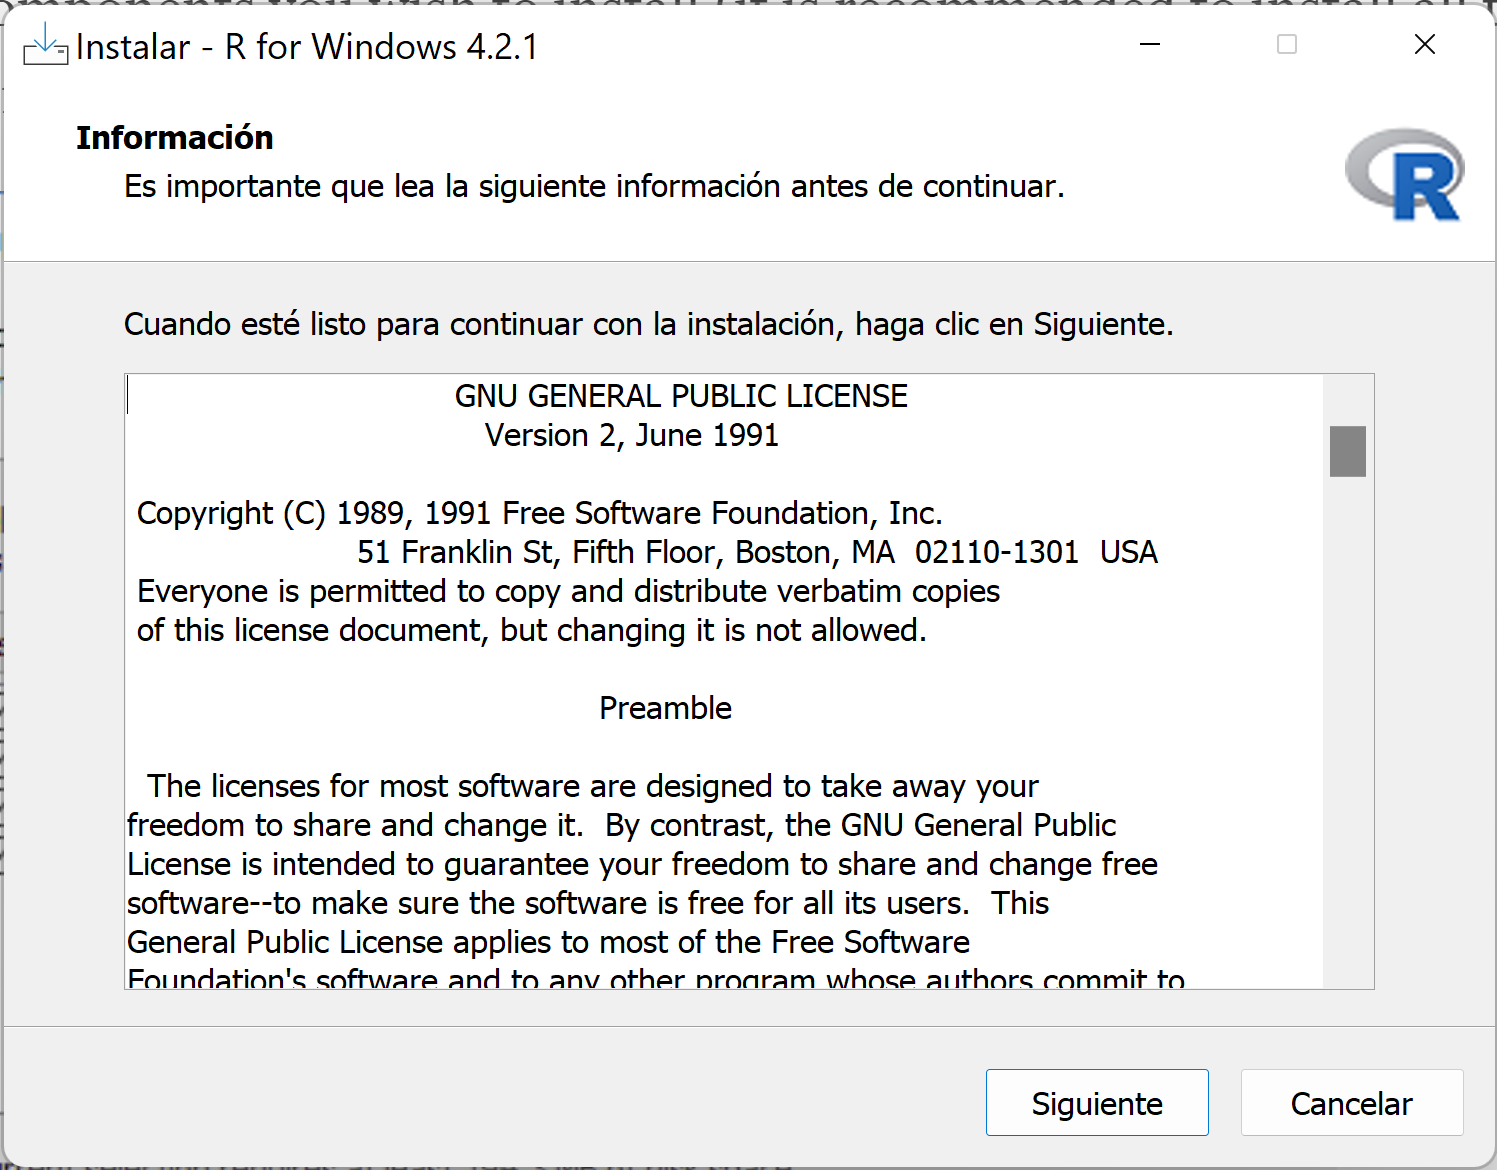
\includegraphics{r-installation/license.png}
            \caption{GNU GENERAL PUBLIC LICENSE.}
            \label{fig:license}
        \end{figure}
    
    \item Select Start Menu folder. Enter the path or select a different folder clicking \textbf{Examinar...} to install R in that folder. Finally click \textbf{Siguiente}.
        \begin{figure}[H]
            \centering
            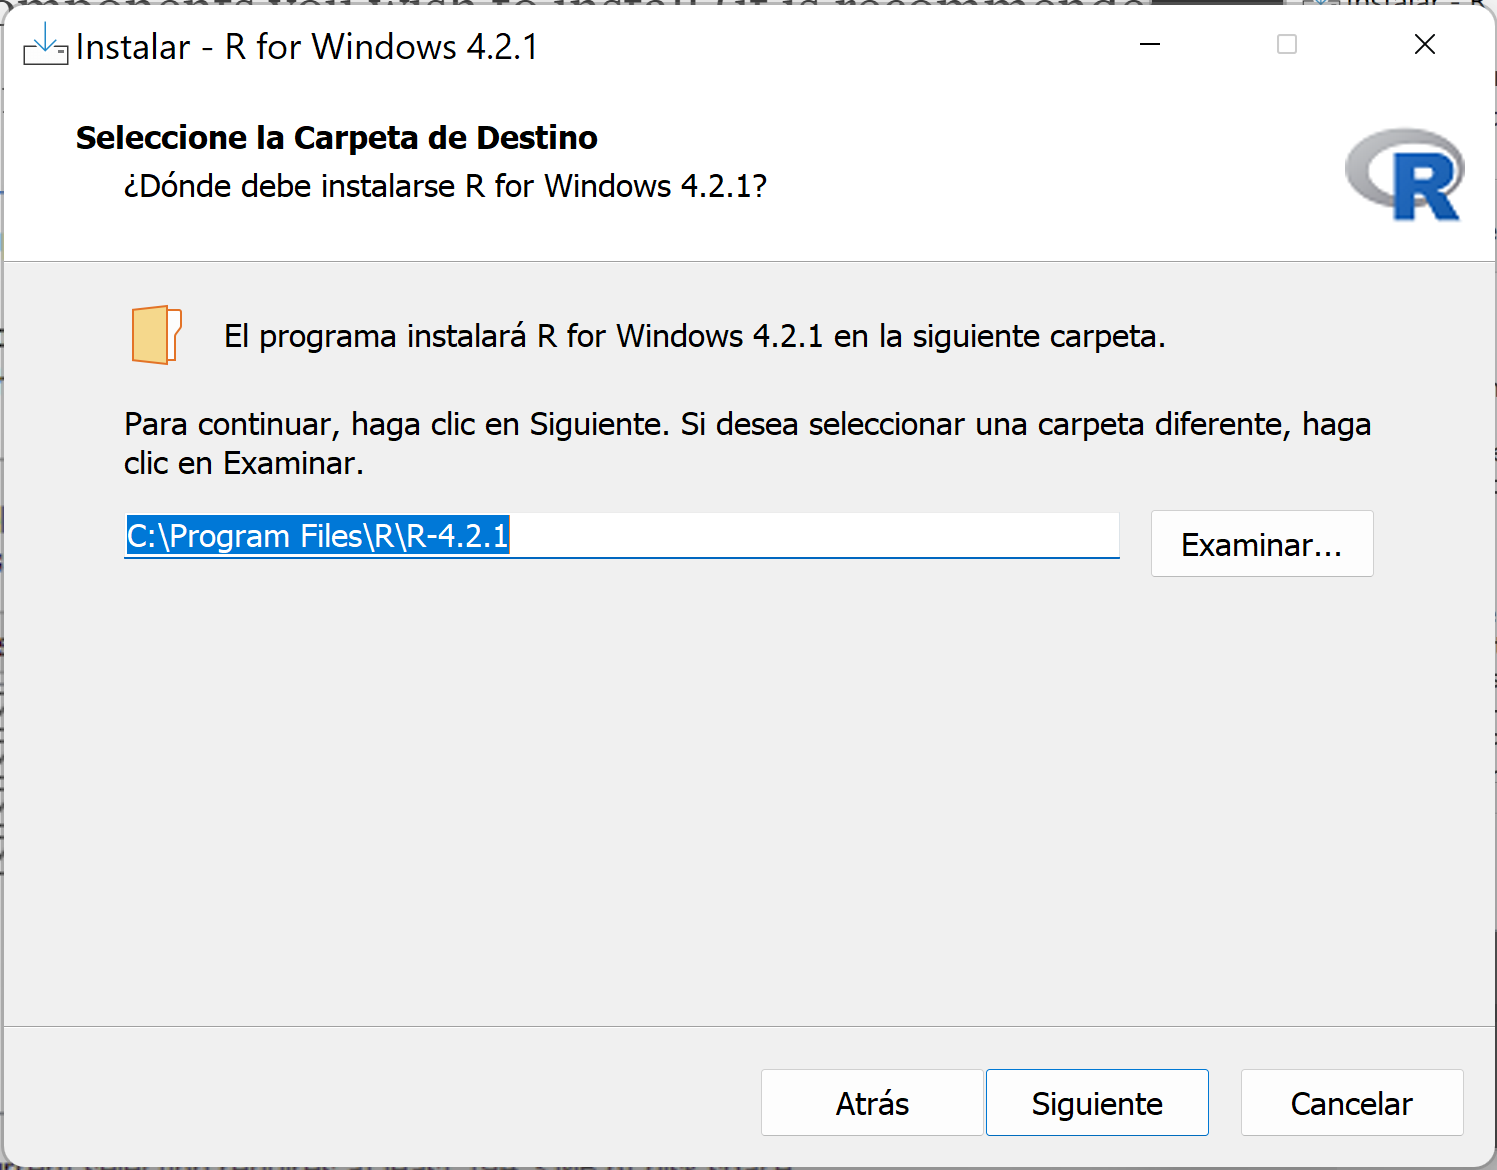
\includegraphics{r-installation/folder.png}
            \caption{Start Menu folder.}
            \label{fig:folder}
        \end{figure}
    
    \item Select components. I leave the ones that come by default selected. Click \textbf{Siguiente}.
        \begin{figure}[H]
            \centering
            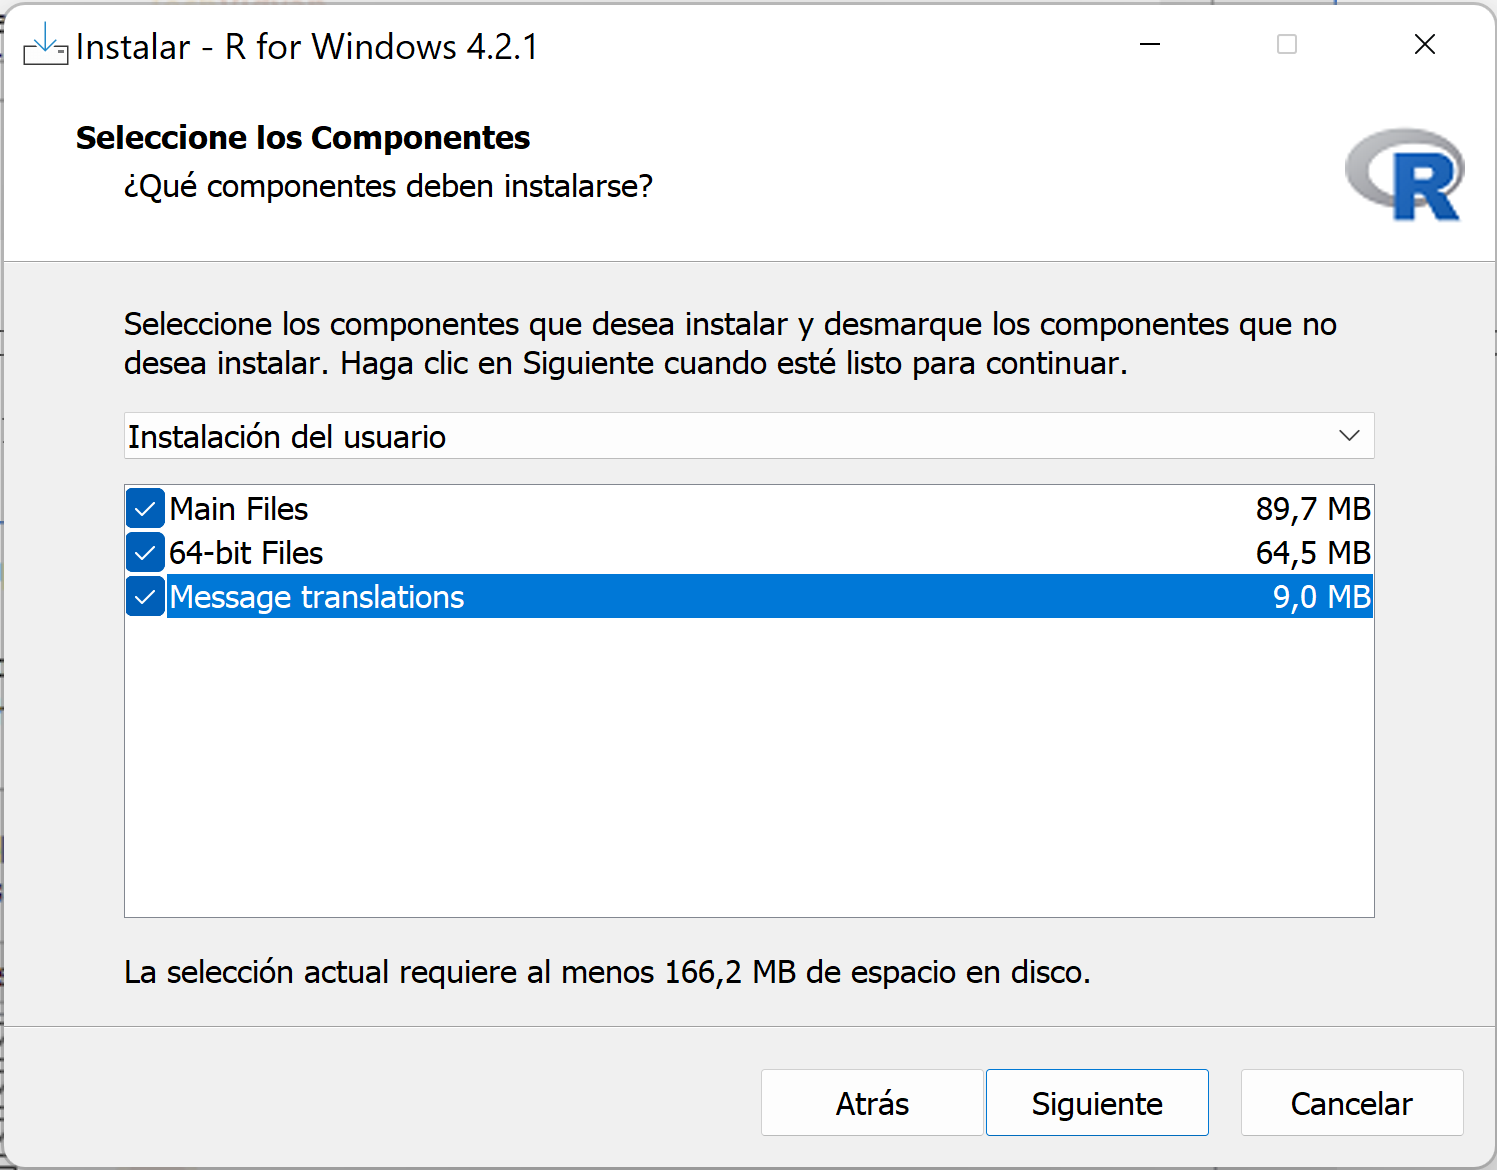
\includegraphics{r-installation/components.png}
            \caption{Select components.}
            \label{fig:components}
        \end{figure}
    
    \item Choose configuration options if you want. It is not necessary. Select \textbf{No} option and click \textbf{Siguiente}.
        \begin{figure}[H]
            \centering
            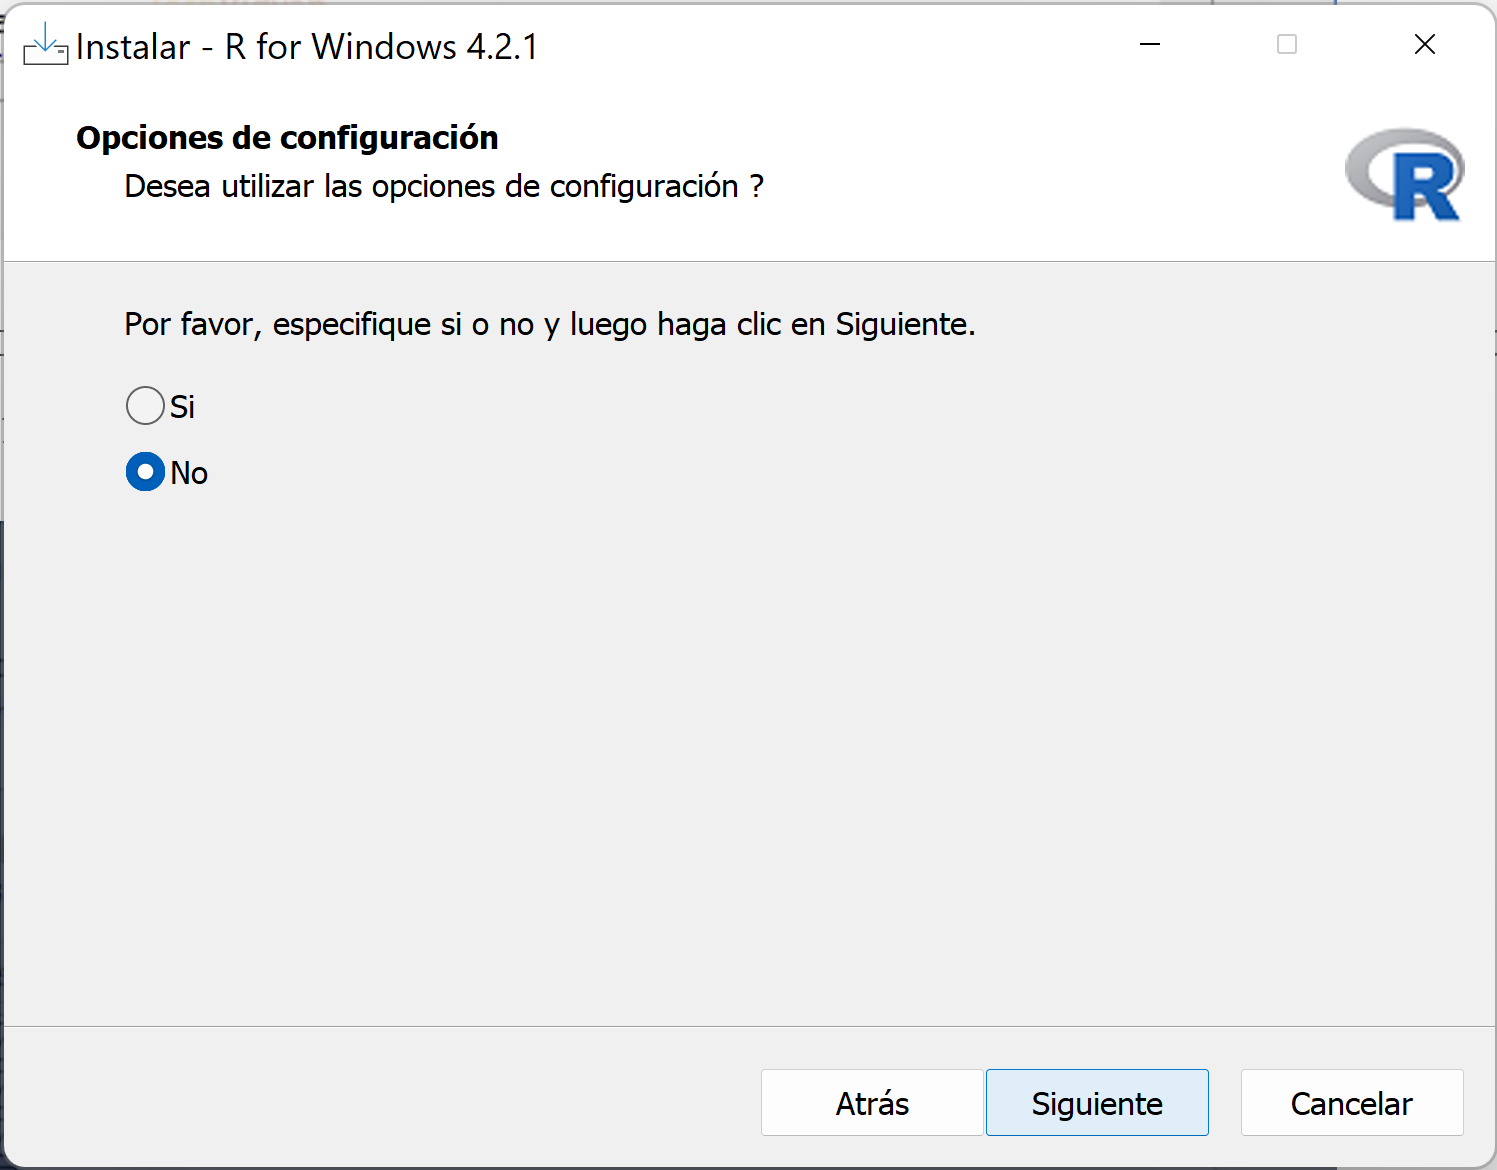
\includegraphics{r-installation/options.png}
            \caption{Configuration options.}
            \label{fig:options}
        \end{figure}
    
    \item Select Additional Tasks. I have selected the options to create a desktop shortcut, to save version number in registry and to associate R with .RData files. Click \textbf{Siguiente} at the end.
        \begin{figure}[H]
            \centering
            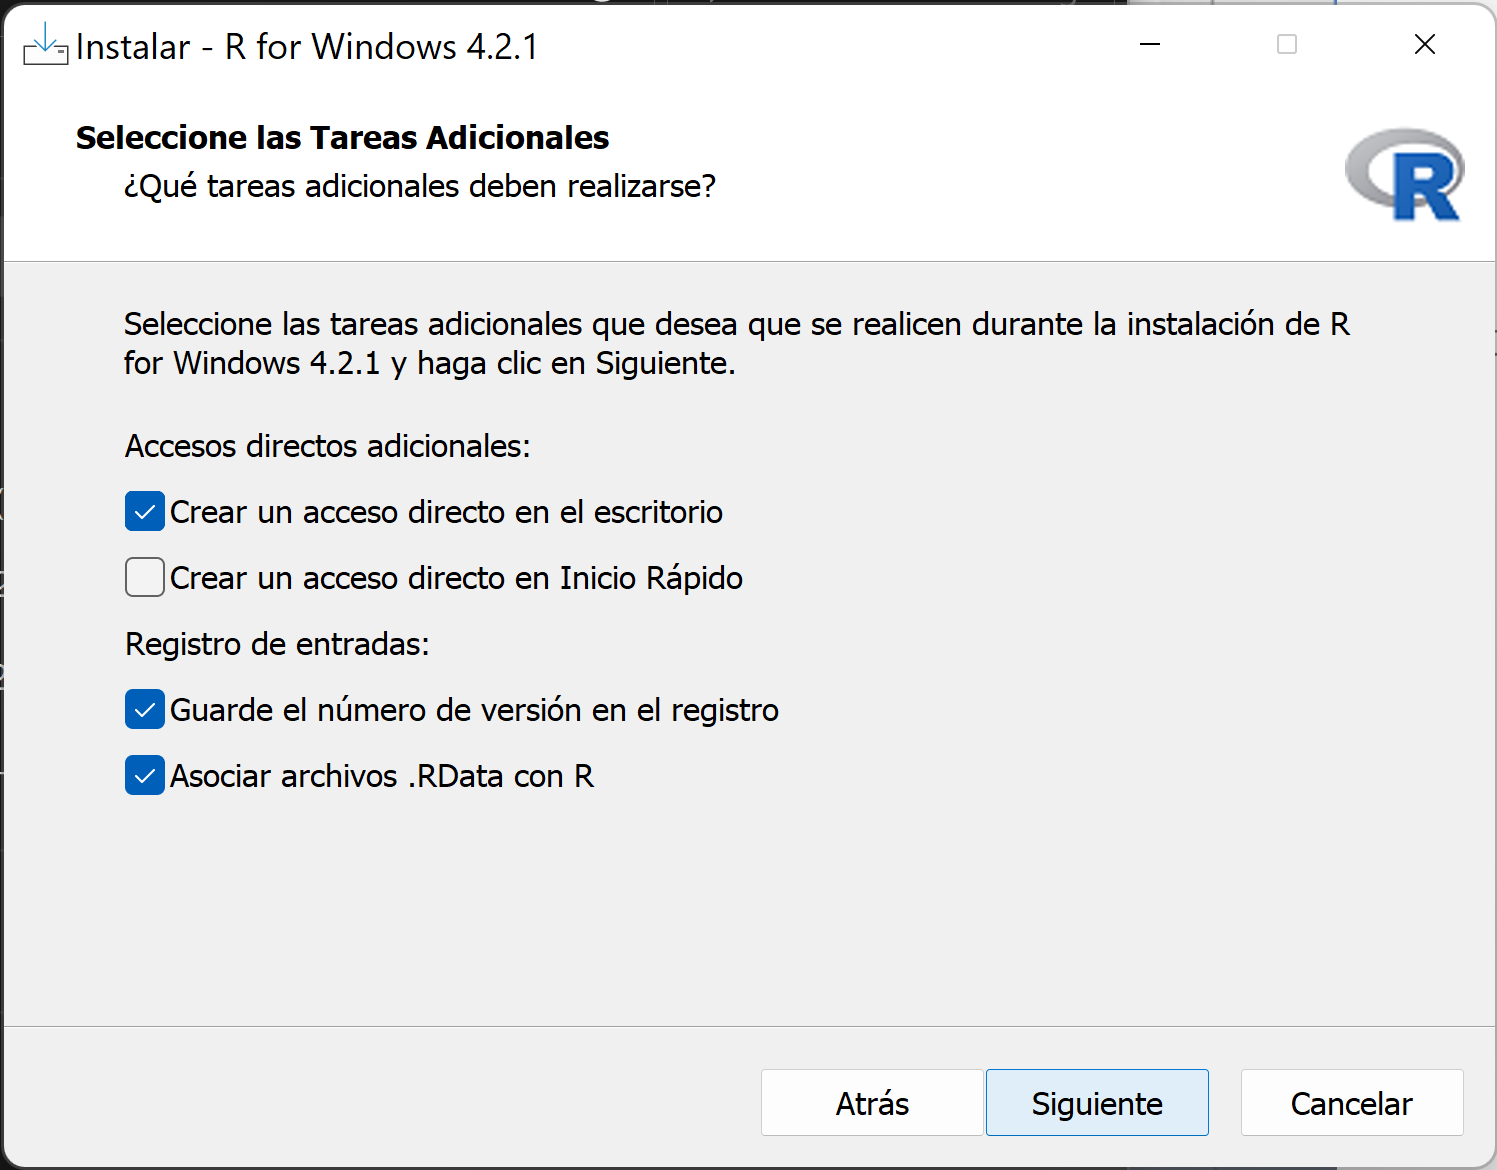
\includegraphics{r-installation/tasks.png}
            \caption{Additional Tasks.}
            \label{fig:tasks}
        \end{figure}
    
    \item Wait for the installation process to complete.
        \begin{figure}[H]
            \centering
            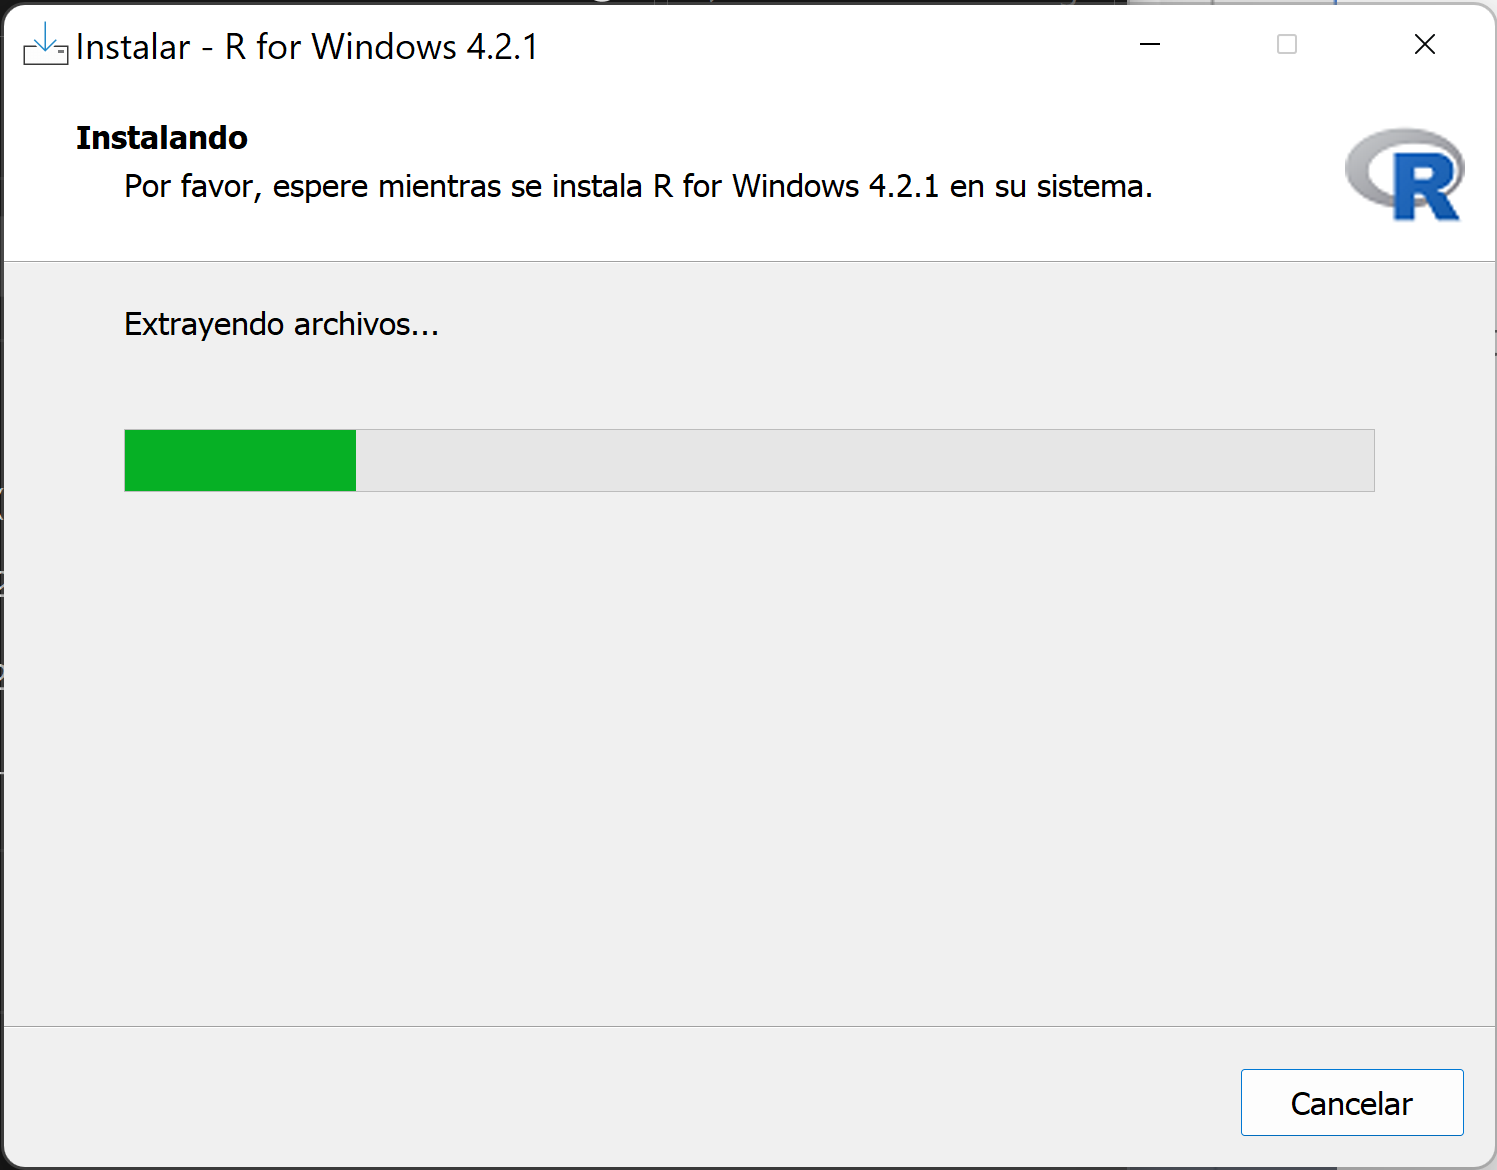
\includegraphics{r-installation/install.png}
            \caption{Installation process.}
            \label{fig:install}
        \end{figure}
    
    \item Click on \textbf{Finalizar} to complete the installation.
        \begin{figure}[H]
            \centering
            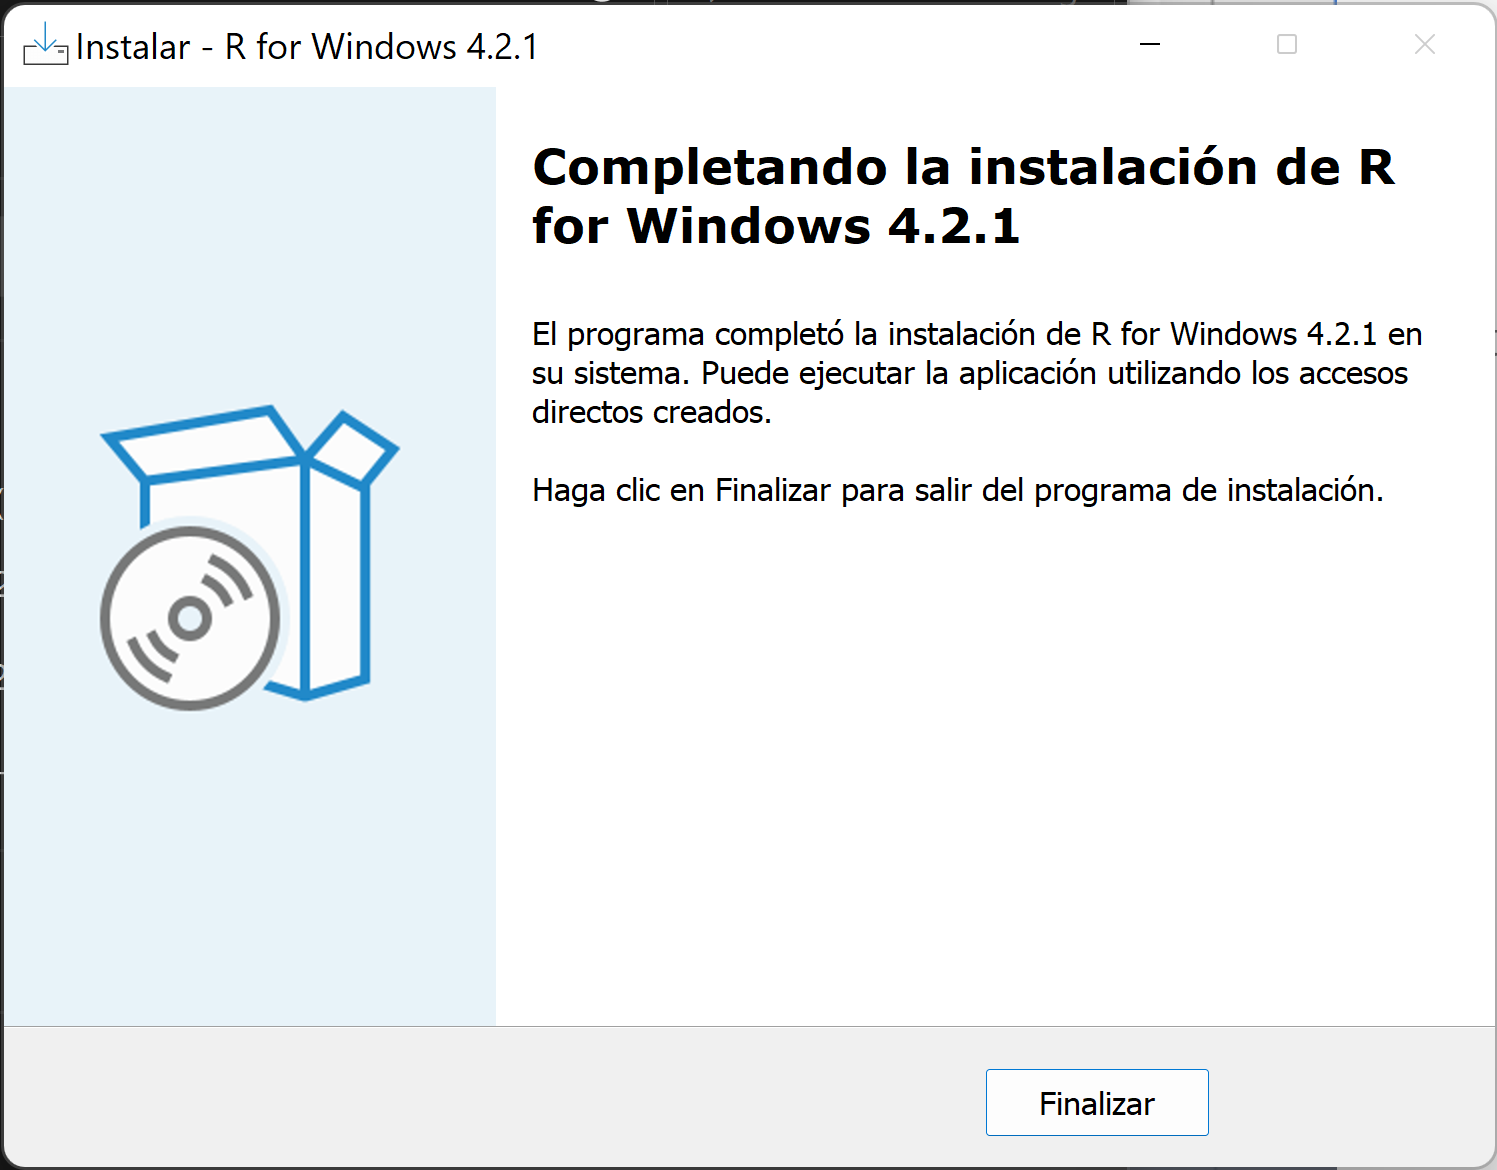
\includegraphics{r-installation/finish.png}
            \caption{Installation completed.}
            \label{fig:finish}
        \end{figure}
\end{enumerate}

\section{RStudio installation}

To install RStudio follow the next steps:

\begin{enumerate}
    \item Go to \href{https://www.rstudio.com/products/rstudio/download/}{download RStudio} website and find RStudio Desktop version. Click \textbf{Download} underneath.
        \begin{figure}[H]
            \centering
            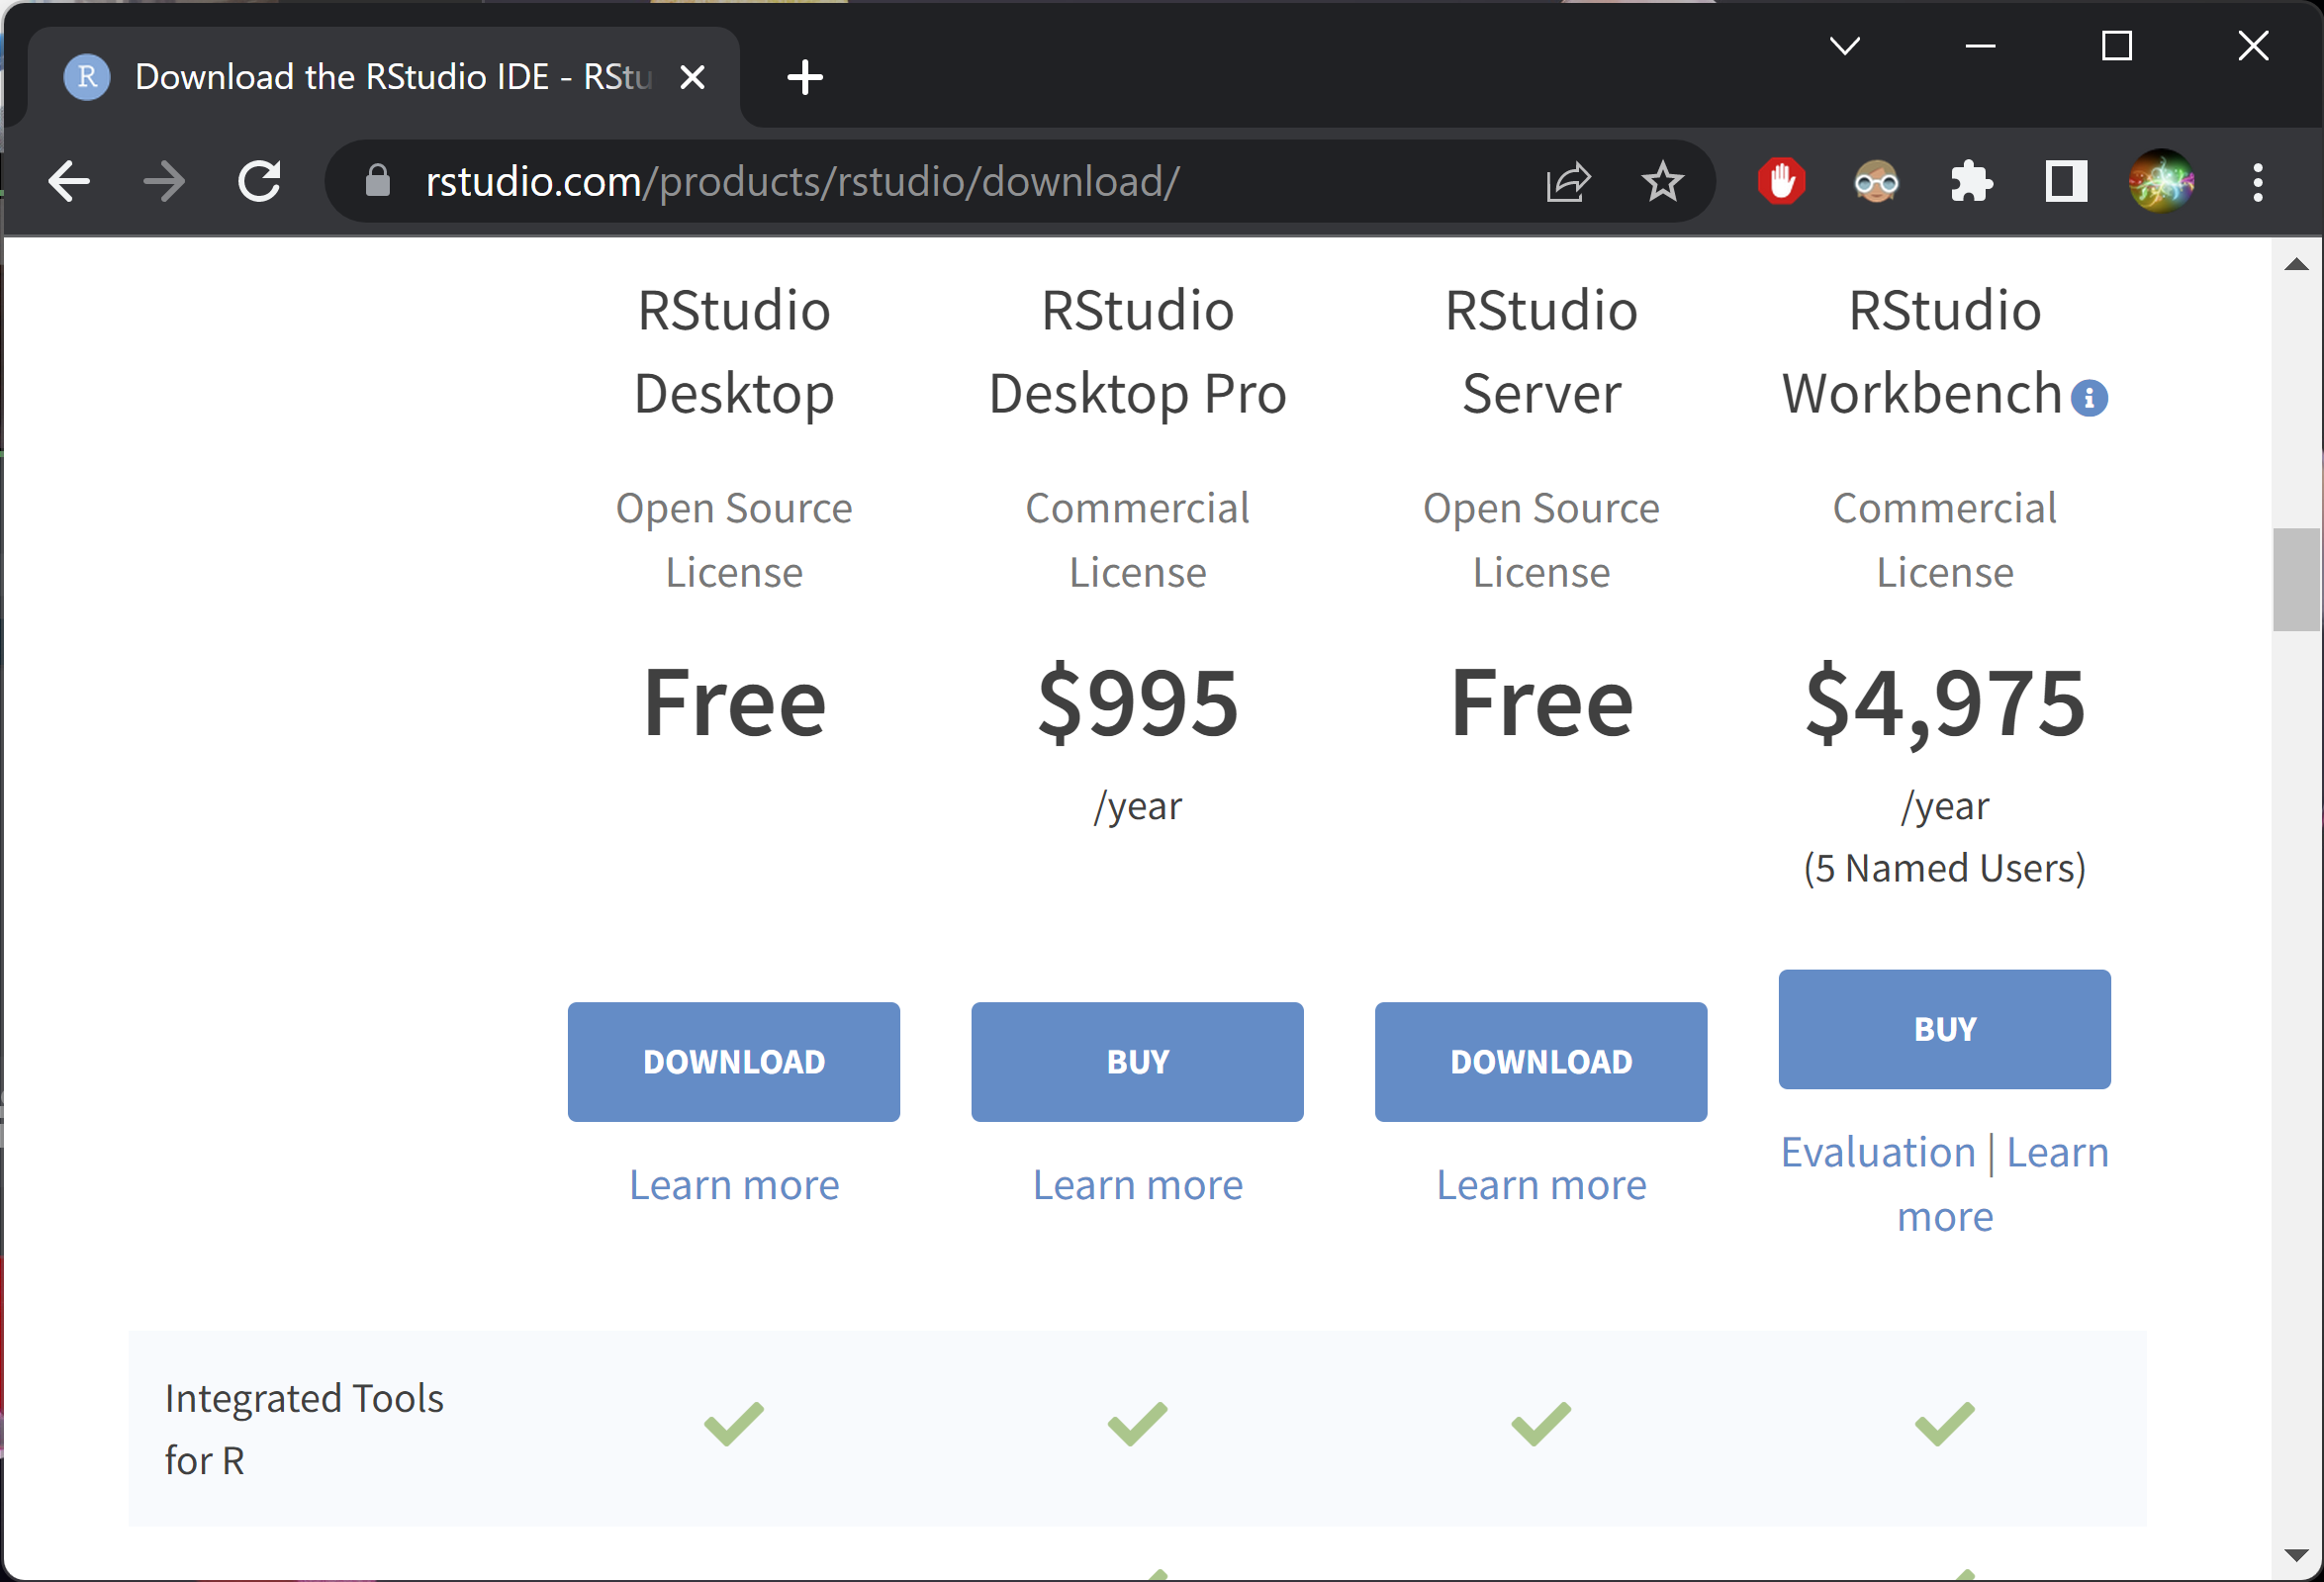
\includegraphics[scale=0.5]{r-installation/download-rs.png}
            \caption{Download RStudio website.}
            \label{fig:download-rs}
        \end{figure}
    
    \item Click on \textbf{Download RStudio for Windows} to get .exe file.
        \begin{figure}[H]
            \centering
            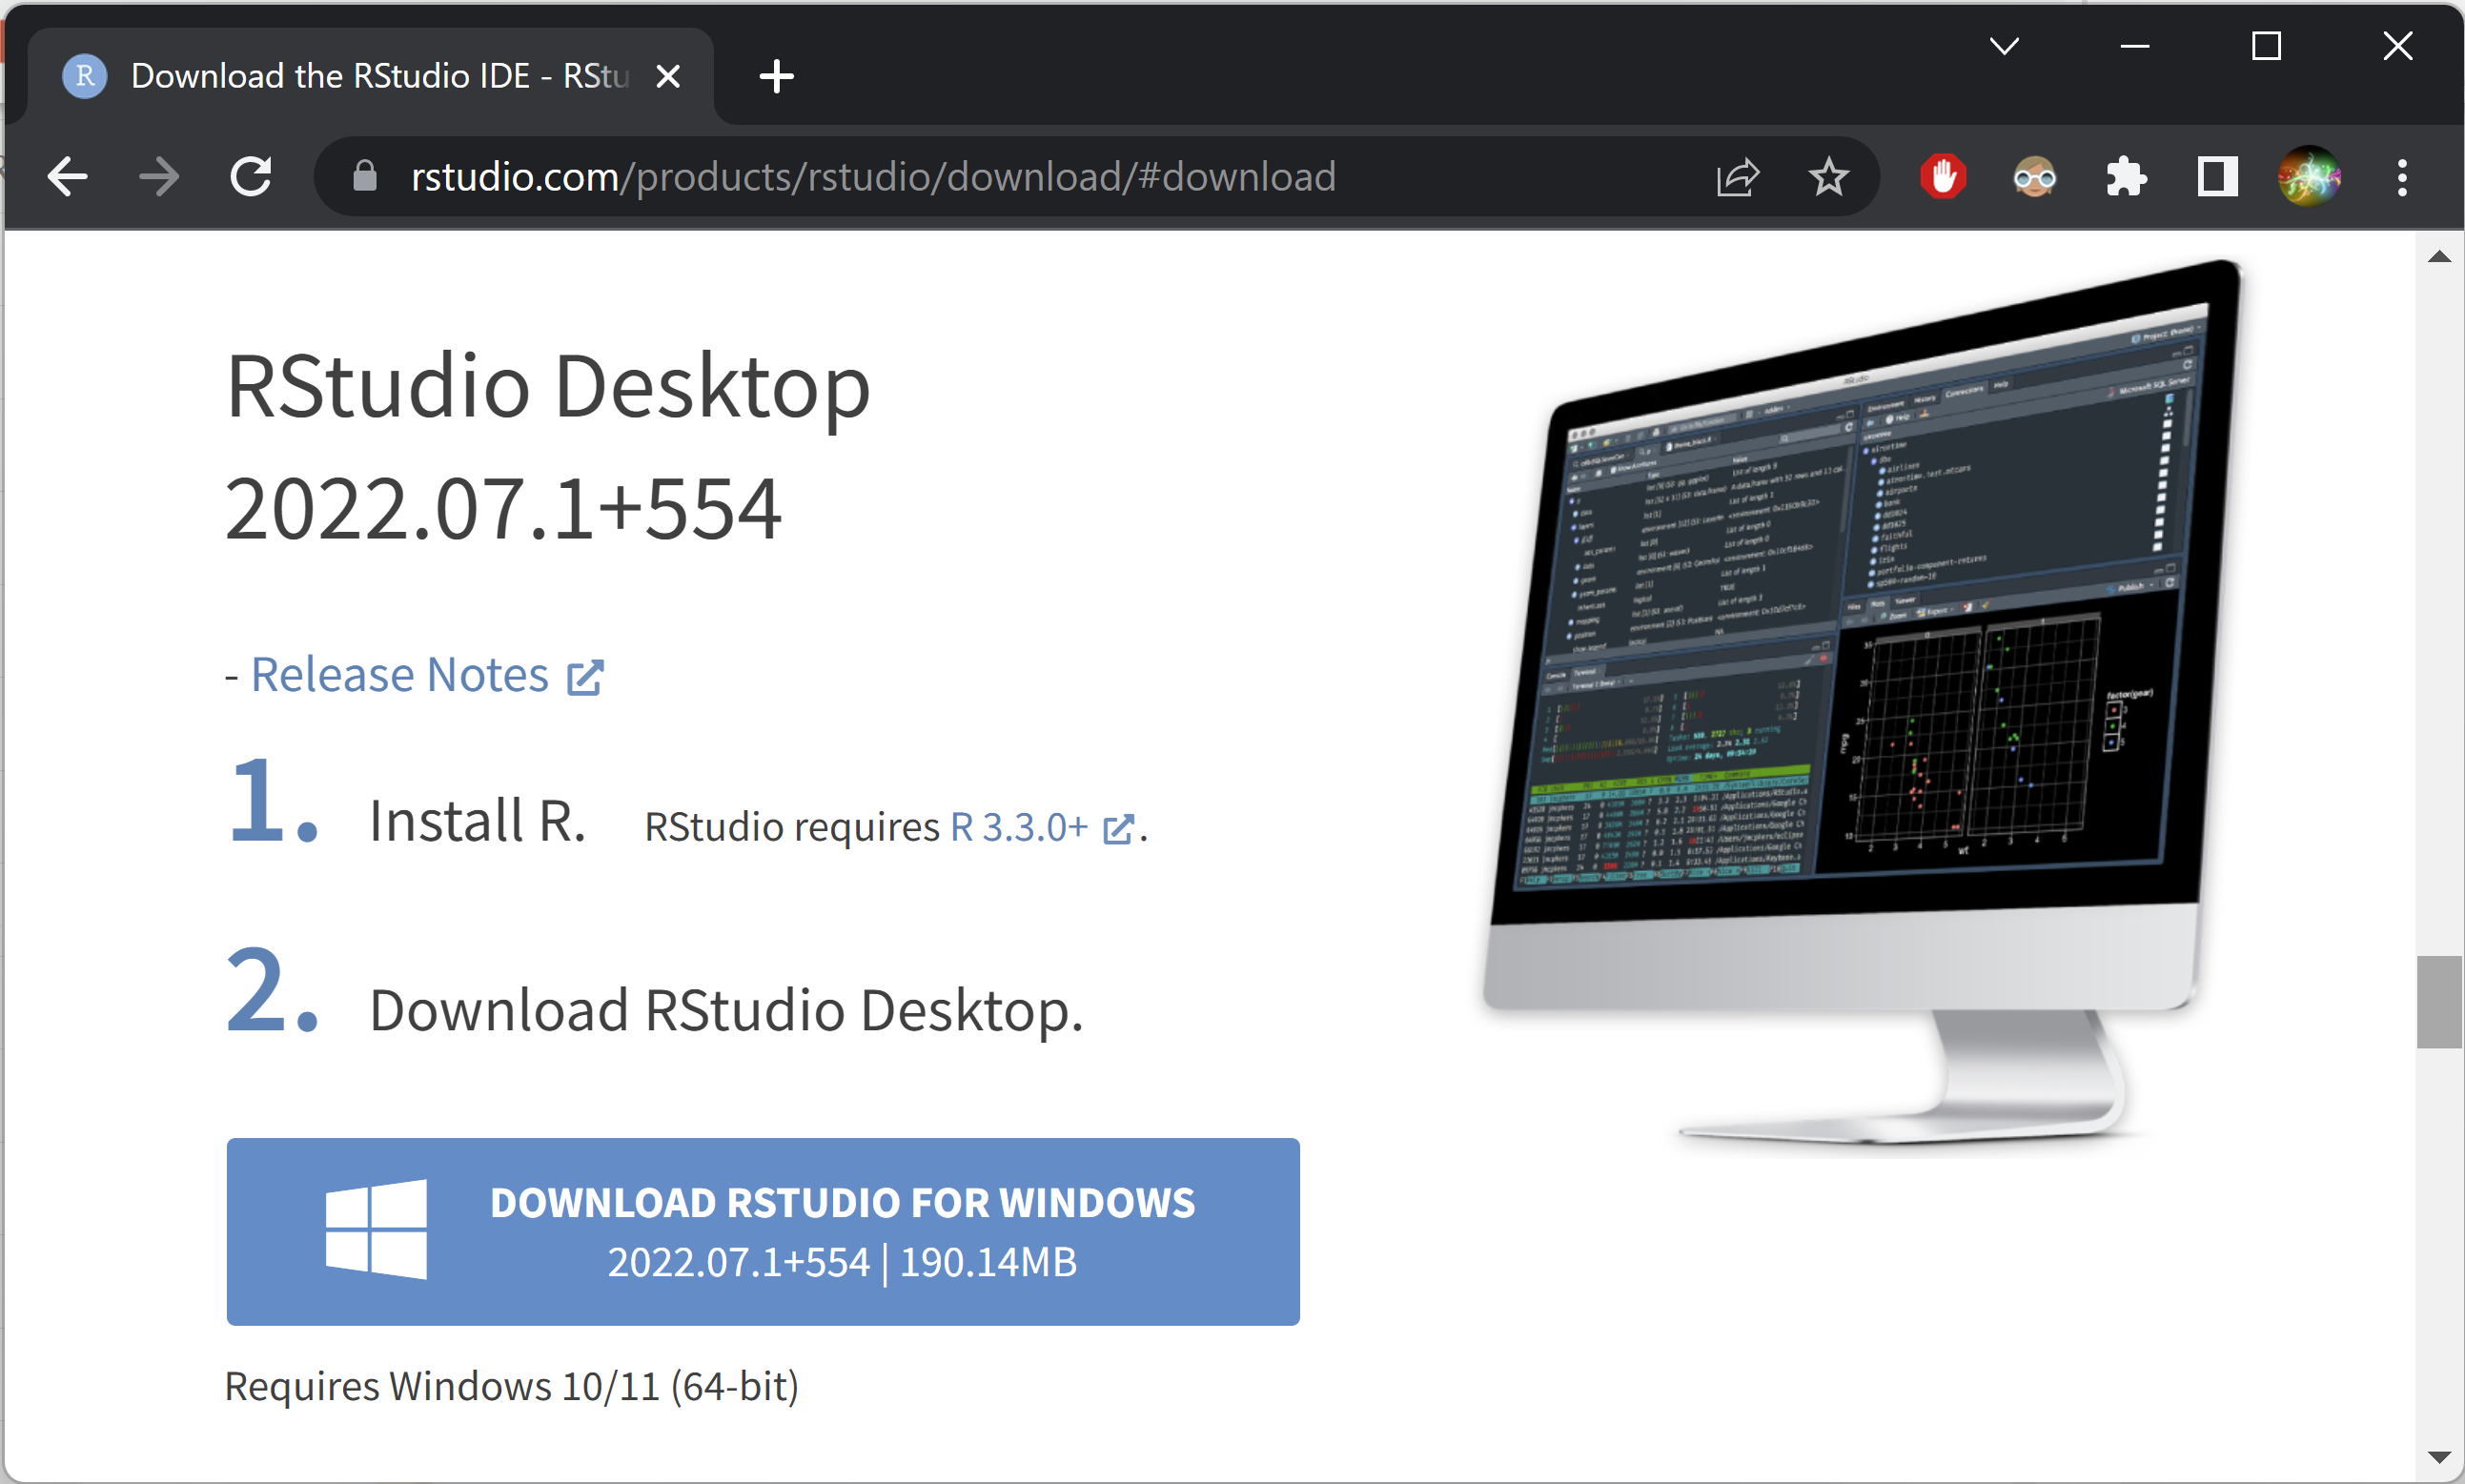
\includegraphics[scale=0.5]{r-installation/download-rs-w.png}
            \caption{Download RStudio for Windows.}
            \label{fig:download-rs-w}
        \end{figure}
    
    \item Run the .exe and follow the installation instructions.
    
    \item Click \textbf{Siguiente} to continue with the installation.
        \begin{figure}[H]
            \centering
            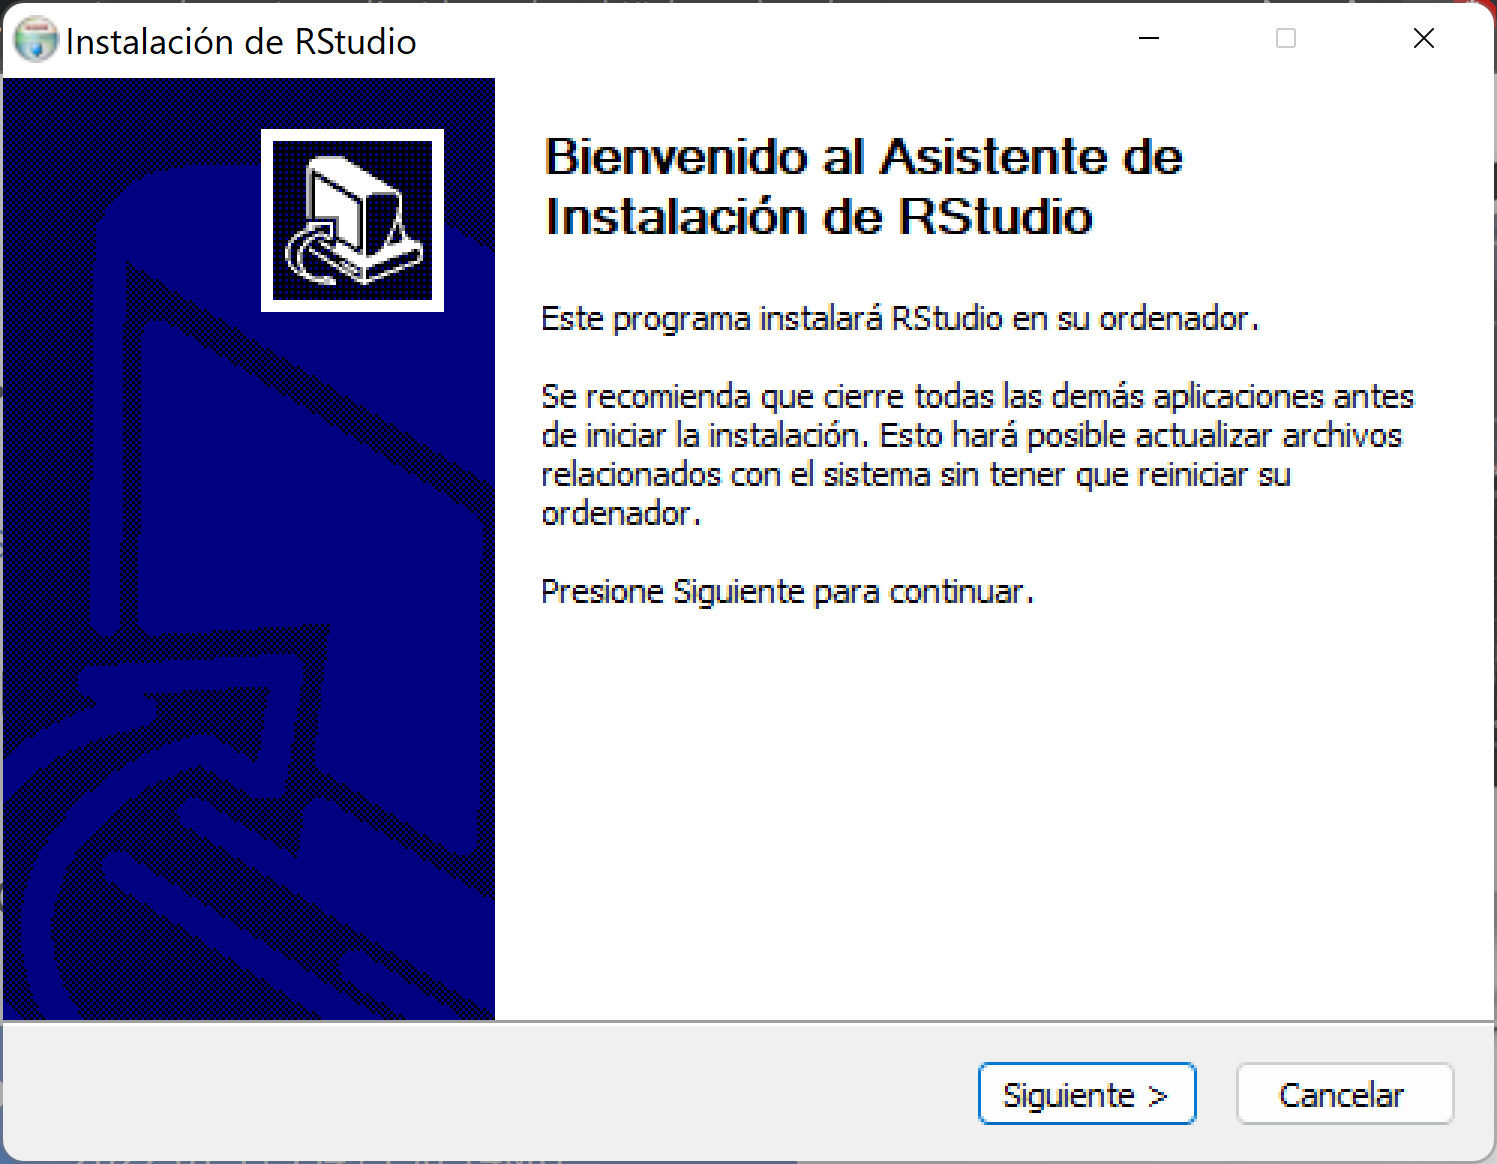
\includegraphics{r-installation/rs-installation.png}
            \caption{Continue with the installation.}
            \label{fig:rs-installation}
        \end{figure}
    
    \item Choose the path to install RStudio. The default path is the one that appears in Figure \ref{fig:path-rs}.
        \begin{figure}[H]
            \centering
            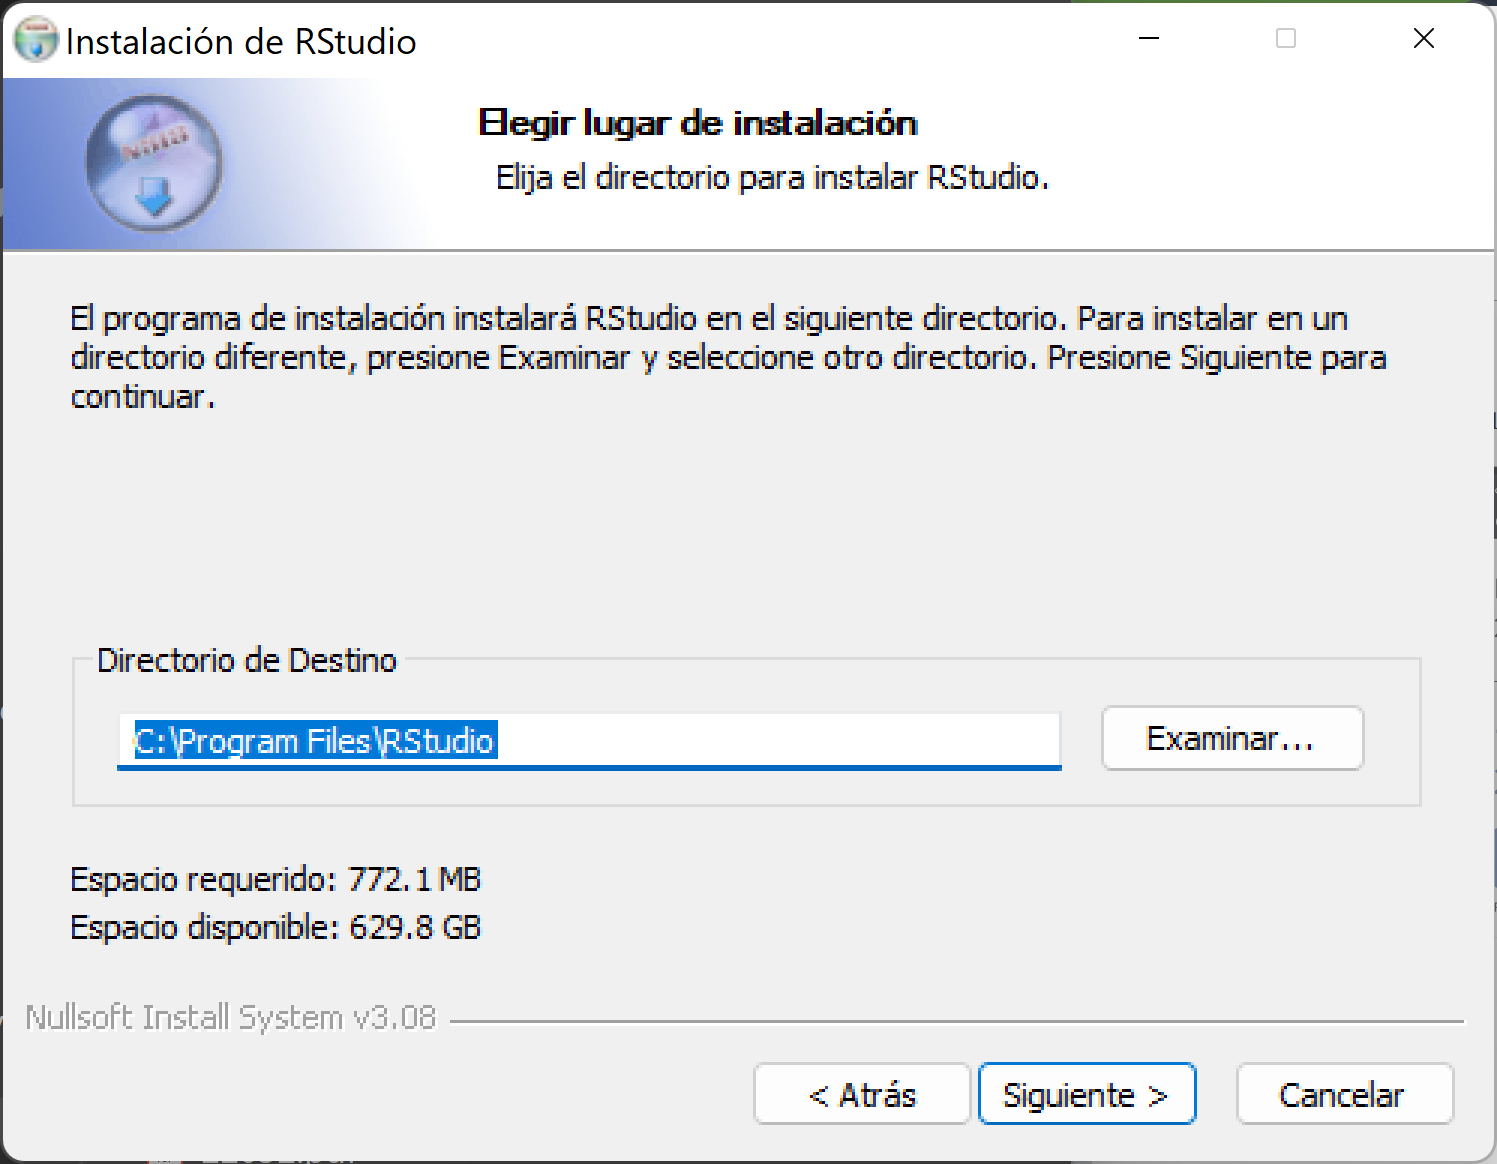
\includegraphics{r-installation/path-rs.png}
            \caption{Choose the path.}
            \label{fig:path-rs}
        \end{figure}
    
    \item Wait for RStudio installation.
        \begin{figure}[H]
            \centering
            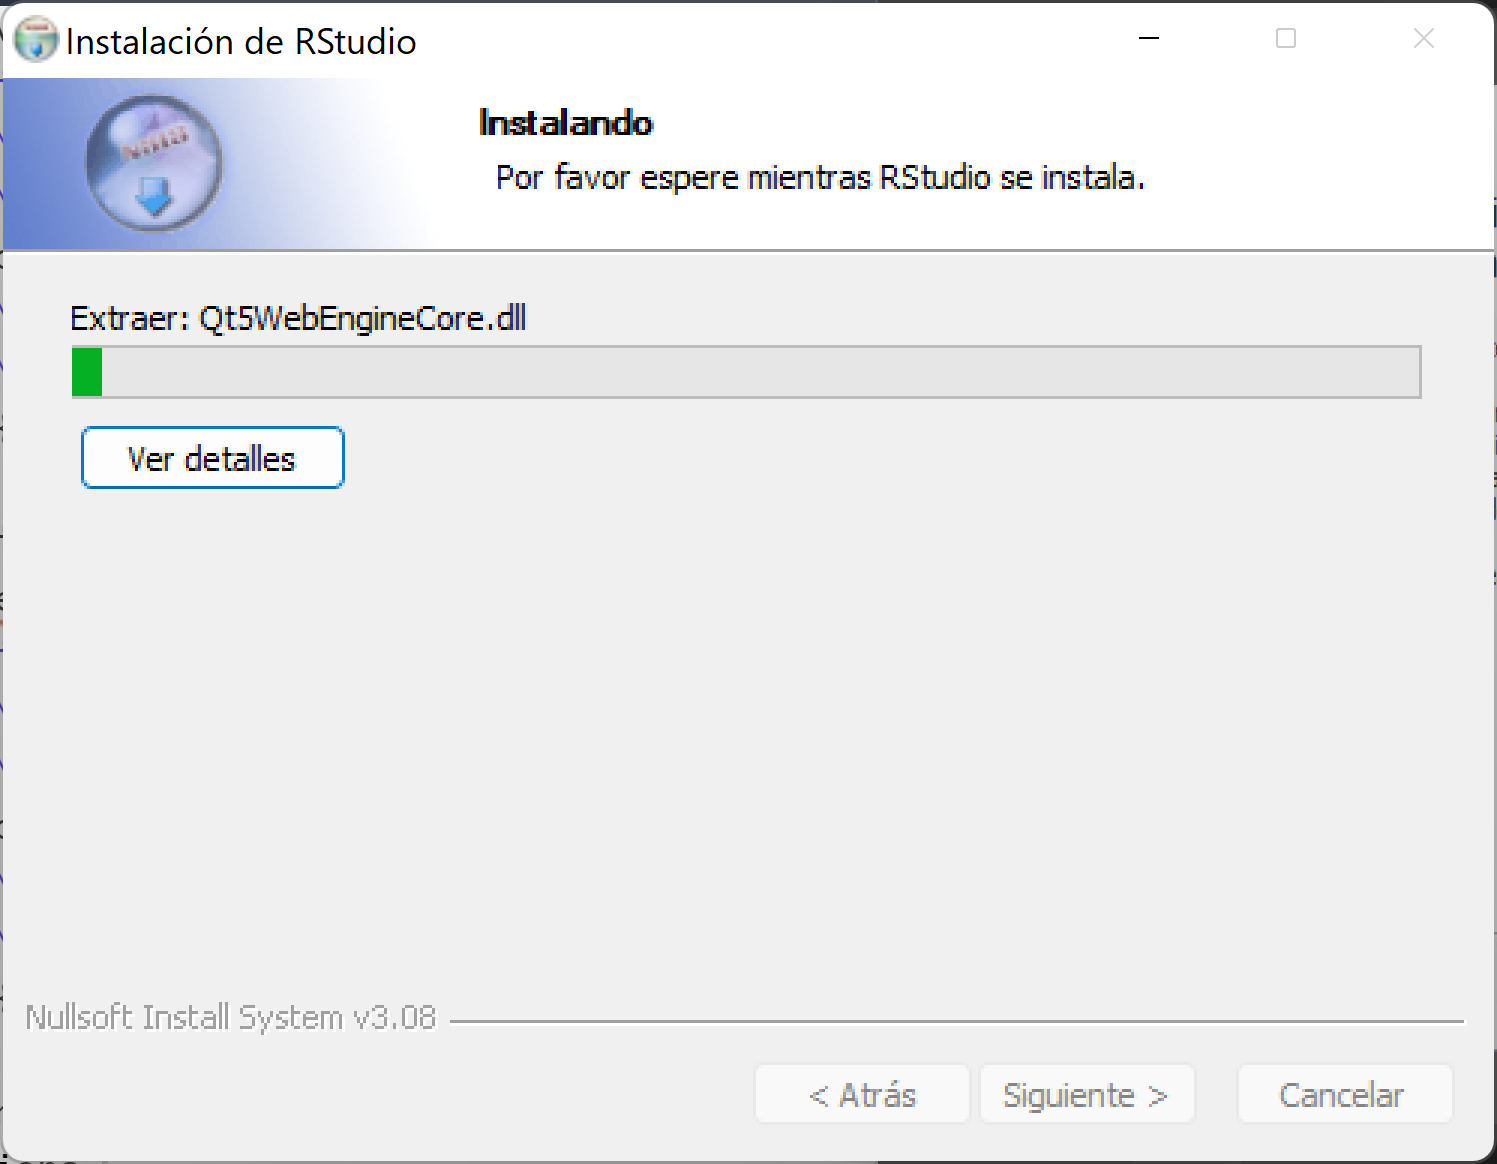
\includegraphics{r-installation/install-rs.png}
            \caption{RStudio installation.}
            \label{fig:install-rs}
        \end{figure}
    
    \item Click on \textbf{Terminar} to complete the installation.
        \begin{figure}[H]
            \centering
            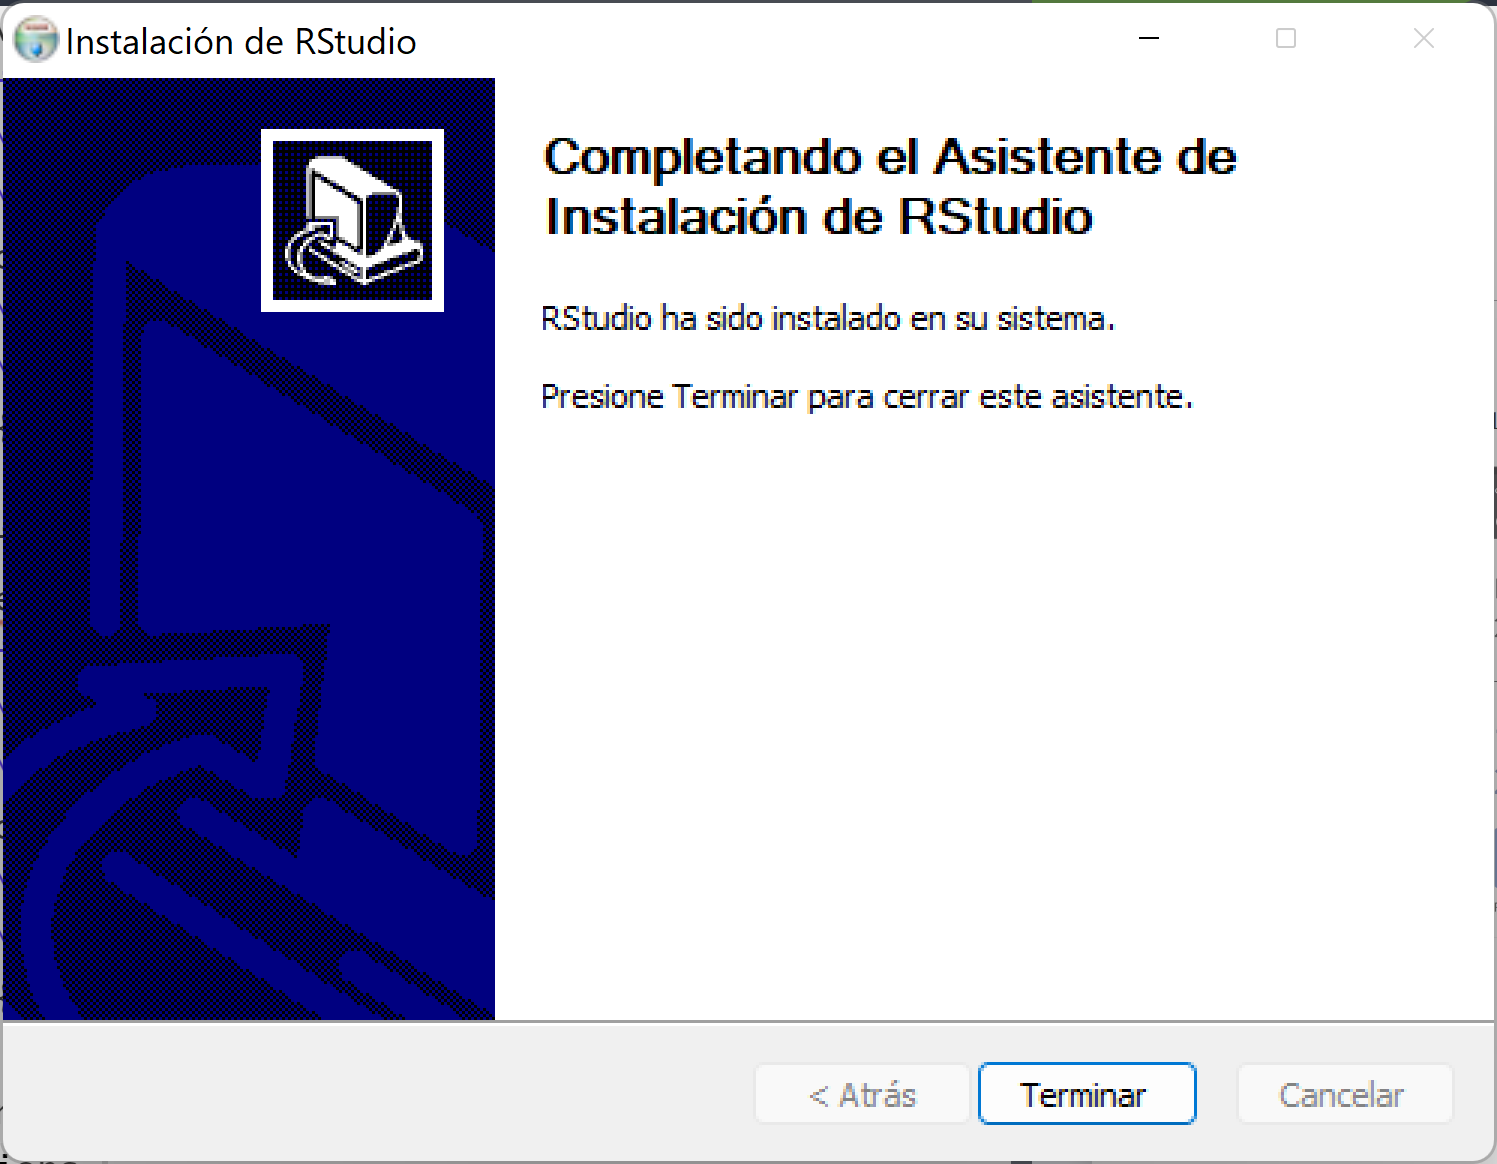
\includegraphics{r-installation/finish-rs.png}
            \caption{Installed.}
            \label{fig:finish-rs}
        \end{figure}
\end{enumerate}